\graphicspath{ {Figures/technology_stack/} }
\chapter{Τεχνολογίες}\label{ch:Development Stack}
\section{Back-End}
	\subsection{Cloud}
	\subsubsection{Ευκαιρίες και προκλήσεις στον τομέα υγείας}
	Πρόσφατες έρευνες έδειξαν ότι το 75\% των διευθυντών πληροφοριακών συστημάτων ανέφεραν ότι θα χρειαστεί να χρησιμοποιήσουν τις τεχνολογίες του υπολογιστικού νέφους στο άμεσο μέλλον \cite{danekCanadaCloud}\cite{cloudComputingIncrease}. Στον τομέα υγείας πολλοί οργανισμοί, διευθυντές και ειδικοί του χώρου πιστεύουν ότι η τεχνολογία του υπολογιστικού νέφους μπορεί να βελτιώσει σημαντικά τις παρεχόμενες υπηρεσίες υγείας, ενώ παράλληλα να μειώσει αισθητά τα λειτουργικά κόστη\cite{Dudley2010}\cite{Schweitzer2012}\cite{Blumenthal2009}\cite{Kabachinski2011}. Επιπλέον μια αναφορά από τον Ευρωπαϊκό Οργανισμό για την Ασφάλεια Δικτύων και Πληροφοριών (ΕΝΙΣΑ) προβλέπει ότι ο νέος αυτός τεχνολογικός τομέας θα λάβει τεράστιες επενδύσεις στο χώρο της υγείας\cite{bannermanCloud}. 

Παρακάτω στο \ref{tab:health_cloud_challenges_opportunities} βλέπουμε σε μορφή πίνακα μια σύνοψη των ευκαιριών αλλά και των προκλήσεων που παρουσιάζει η τεχνολογία του υπολογιστικού νέφους για το χώρο της υγείας.
	
\begin{table}[H]
	\begin{center}
	    \begin{tabular}{|l| p{\dimexpr 0.45\linewidth-2\tabcolsep} | p{\dimexpr 0.45\linewidth-2\tabcolsep} |}
	    \hline
	    \rowcolor{grayy}
	    \textbf{Τομέας} & \textbf{Ευκαιρείες} & \textbf{Προκλήσεις}
	    \\ \hline    
	    \multirow{3}{*}{Διοίκησης} & Χαμηλότερο κόστος υποδομών του IT & Έλειψη εμπιστοσύνης των προμηθευτών υγείας \\
	    & Διάθεση υπολογιστικών πόρων on demand & Οργανωτική αδράνεια \\
	    & Σταδιακή πληρωμή ανάλογως τις ανάγκες & Απώλεια άμέσου ελέγχου δεδομένων \\ \hline
	    \multirow{3}{*}{Τεχνολογίας} & Μείωση εργασιών συντήρησης του ΙΤ & Προβλήματα εξάντλησης πόρων \\
	    & Ευελξία και επεκτασιμότητα υποδομών IT & Απρόβλεπτη συμπεριφορά \\
	    & Οικολογική λύση & Απώλεια άμέσου ελέγχου δεδομένων  \\ \hline
	    \multirow{3}{*}{Ασφάλειας} & Περισσότεροι πόροι για προστασία δεδομένων & Κατάχρηση προνομίων \\
	    & Αντιγραφή των δεδομένων σε πολλαπλές τοποθεσίες & Ασφάλεια των φυσικών αποθηκευτικών μέσων \\
	    & Δυναμικά επεκτάσιμοι πόροι ασφάλεια που αυξάνει την ελαστικότητα & Προβλήματα διαχείρησης κλειδιών κρυπτογράφησης \\ \hline
	    \end{tabular}
	    \caption{Ευκαιρείες και Προκλήσεις cloud στον χώρο της υγείας}
	    \label{tab:health_cloud_challenges_opportunities}
	\end{center}
\end{table}	
	\subsubsection{Θεωρητικό υπόβαθρο υπολογιστικού νέφους}
	To cloud computing (υπολογιστικό νέφος) όπως ορίζεται από το NIST (Εθνικό Ινστιτούτο Προτύπων και Τεχνολογίας)  είναι μια τεχνολογία, η οποία επιτρέπει την πρόσβαση από παντού, παρέχει μετά από αίτημα πρόσβαση στο δίκτυο για την κοινή χρήση προσαρμοστικών υπολογιστικών πόρων (π.χ., δίκτυα, servers, συστήματα αποθήκευσης, εφαρμογές και υπηρεσίες), μπορεί να ξεκινήσει και να αναπτυχθεί γρήγορα με ελάχιστη διαχείριση και χωρίς καμία αλληλεπίδραση με τον φορέα παροχής υπηρεσιών. \cite{cloudComputing} Το cloud computing παρέχει στους χρήστες και στις επιχειρήσεις διάφορες δυνατότητες για την αποθήκευση και την επεξεργασία των δεδομένων τους σε τρίτα κέντρα δεδομένων. \cite{Haghighat2015}
	
	Το cloud computing ουσιαστικά στηρίζεται στην κατανομή των πόρων με στόχο την επίτευξη συνοχής και οικονομίας μέσω ενός δικτύου και την μεγιστοποίηση της απόδοσης τους. Οι πόροι του cloud δεν είναι μόνο διαμοιραζόμενοι από πολλούς χρήστες αλλά μπορούν και να ανακατανεμηθούν δυναμικά ανάλογα με την ζήτηση, γεγονός που μπορεί να χρησιμοποιηθεί όταν κατανέμονται στους διάφορους χρήστες.  Για παράδειγμα, μια cloud εγκατάσταση ηλεκτρονικών υπολογιστών οι οποία εξυπηρετεί Ευρωπαίους χρήστες στην διάρκεια των Ευρωπαϊκών εργάσιμων ωρών μπορεί να ανακατανείμει τους ίδιους πόρους για να εξυπηρετήσει χρήστες στην Βόρεια Αμερική κατά τις εργάσιμες ώρες της Βόρειας Αμερικής σε μία διαφορετική εφαρμογή. Αυτή η προσέγγιση βοηθά στην μεγιστοποίηση της χρήσης της υπολογιστικής ισχύος ενώ ταυτόχρονα μειώνεται το ολικό κόστος των φυσικών πόρων καθώς χρησιμοποιούμε λιγότερη ενέργεια, κλιματισμό κ.λ.π. για να διατηρείται το σύστημα.Με χρήση του cloud computing πολλοί χρήστες μπορούν να έχουν πρόσβαση σε έναν server και να ανακτούν και να ανανεώνουν τα δεδομένα τους χωρίς να αγοράζουν άδειες για όλες τις διαφορετικές εφαρμογές. 
	
	Οι πάροχοι cloud συνήθως χρησιμοποιούν μοντέλο κοστολόγησης "πλήρωσε όσο χρησιμοποιήσεις".  Παρουσιάζει σπουδαιότητα λοιπόν το γεγονός ότι οι "πελάτες" μπορούν να εξοικονομήσουν χρηματικούς πόρους στο πέρασμα του χρόνου, καθώς χρησιμοποιώντας τους πόρους στο cloud, πληρώνουν μόνο για τους πόρους που χρησιμοποιούν και όχι για την αγορά και συντήρηση άφθονων μηχανημάτων (π.χ. εξυπηρετητών). Η λύση λοιπόν του cloud computing λοιπόν αποτελεί μία ιδιαίτερα ελκυστική προοπτική για τους χρήστες στους οποίους η χρήση των πόρων ποικίλλει σημαντικά καθώς και σε αυτούς στους οποίους  η αγορά μηχανημάτων και το κόστος συντήρησης τους αποτελούν σημαντικό τμήμα του προϋπολογισμού. 

	Ένα πλήρες σύστημα υπολογιστικού νέφους αποτελείται από τα εξής βασικά συστατικά : 
	\begin{itemize}
	\item Πελάτες - υπολογιστές. Πρόκειται για τις συσκευές των τελικών χρηστών μέσω των οποίων αποκτούν πρόσβαση στο υπολογιστικό νέφος. Χωρίζονται σε τρεις κατηγορίες: τις κινητές συσκευές (mobile devices) που επιτρέπουν στον χρήστη την απομακρυσμένη πρόσβαση μετά από επεξεργασία του κατανεμημένου διακομιστή, τους παχείς πελάτες (thick clients) που είναι οι σταθεροί υπολογιστές ή τα λάπτοπ τα οποία συνδέονται στο cloud με χρήση ενός φυλλομετρητή και τους λεπτούς πελάτες (thin clients ) που είναι υπολογιστές με μικρή υπολογιστική ισχύς και χωρίς σκληρούς δίσκους, που εμφανίζουν τα δεδομένα αφού τα επεξεργαστεί πρώτα ο διακομιστής.
	\item Κέντρο δεδομένων. Είναι το σύνολο των διακομιστών, όπου τρέχουν οι εφαρμογές. Στο κέντρο δεδομένων εμπίπτουν και οι εικονικοί διακομιστές (μπορεί σε έναν υπολογιστή να γίνει εγκατάσταση ώστε να επιτρέπεται η ταυτόχρονη ύπαρξη πολλαπλών στιγμιοτύπων από εικονικούς διακομιστές).
	\item Κατανεμημένους διακομιστές. Οι διακομιστές αυτοί βρίσκονται σε διαφορετικές γεωγραφικές θέσεις, έτσι ώστε να εξασφαλίζεται μεγαλύτερη ευελιξία και υψηλότερη ασφάλεια στις παροχές που προσφέρει το cloud computing. Έτσι μπορούν να αντιμετωπιστούν αποτελεσματικά περιπτώσεις παραβίασης ασφάλειας ή ανάγκης επιπλέον αποθηκευτικού χώρου και υπολογιστικής δύναμης.
	\end{itemize}		
	
	Στο σχήμα   \ref{fig:cloud},φαίνεται μία σχηματική αναπαράσταση του συστήματος cloud computing.
	
			\begin{figure}[h]
	    \centering
	    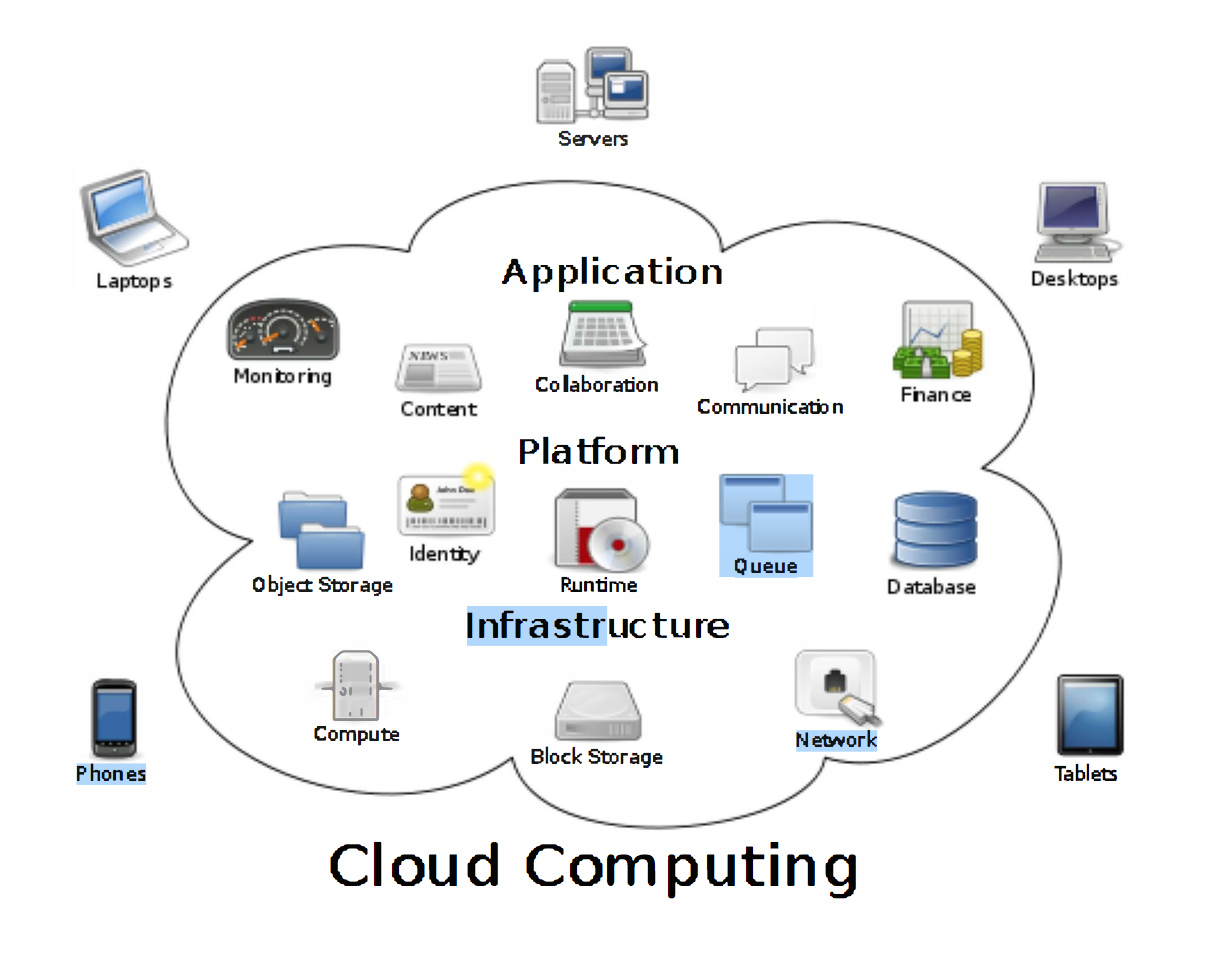
\includegraphics[width=0.7\textwidth]{cloud.png}
	    \caption{ Cloud Computing.  }
	    \label{fig:cloud}
	\end{figure}

		Το μοντέλο cloud αποτελείται από πέντε βασικά χαρακτηριστικά:
		\begin{itemize}
		\item Αυτοεξυπηρέτηση μετά από ζήτηση (On-demand self-service). Ο χρήστης των υπηρεσιών του νέφους μπορεί να χρησιμοποιεί τους υπολογιστικούς πόρους που χρειάζεται, όπως χρόνο στον server και αποθηκευτικό χώρο,  αυτόματα και χωρίς να απαιτείται ανθρώπινη αλληλεπίδραση με τον φορέα παροχής υπηρεσιών. 
		\item Ευρεία πρόσβαση στο δίκτυο (Broad network access). Οι δυνατότητες που προσφέρονται είναι διαθέσιμες μέσω του δικτύου και προσβάσιμες μέσω τυποποιημένων μηχανισμών που προωθούν την χρήση ετερογενών πλατφορμών λεπτών ή παχέων πελατών (π.χ., κινητά τηλέφωνα, τάμπλετ, υπολογιστές). 
		\item Διάθεση των πόρων. Οι υπολογιστικοί πόροι των cloud παρόχων είναι συγκεντρωμένοι με χρήση ενός μοντέλου πολλαπλών ενοικιαστών (κάθε οργανισμός εργάζεται με ένα προσαρμοσμένο εικονικό στιγμιότυπο της εφαρμογής) έτσι ώστε να  μπορούν να ανατεθούν οι φυσικοί και εικονικοί πόροι ανάλογα με την ζήτηση των καταναλωτών. Οι παρεχόμενοι πόροι μπορεί να περιλαμβάνουν πόρους όπως μνήμη, επεξεργαστική ισχύ, εύρος δικτύου, εικονικές μηχανές.
		\item Μεγάλη ελαστικότητα (Rapid Elasticity). Οι δυνατότητες του cloud computing παρέχονται με μεγάλη ταχύτητα και προσαρμοστικότητα , ώστε να είναι σε θέση να κλιμακώνουν πολύ γρήγορα ανάλογα με την ζήτηση που υπάρχει και να φαίνονται απεριόριστες σε οποιαδήποτε ποσότητα και χρονική στιγμή ζητηθούν. 
		\item Μετρούμενη υπηρεσία (Measured Service). Τα cloud computing συστήματα πραγματοποιούν μετρήσεις, σε συγκεκριμένα επίπεδα αφαίρεσης ανάλογα με το είδος της υπηρεσίας (επεξεργασία, μνήμη, ενεργοί λογαριασμοί χρηστών). Με βάση αυτές τις μετρήσεις γίνεται έλεγχος και ενέργειες για την βελτιστοποίηση της χρήσης των πόρων. Επιπλέον η χρήση των πόρων παρακολουθείται, ελέγχεται και καταγράφεται με αποτέλεσμα την παροχή διαφάνειας μεταξύ του χρήστη και του παρόχου του cloud.
		\end{itemize}	\cite{characteristicsCloud}\cite{nist}.

Το cloud computing μπορεί να διαχωριστεί με βάση τις υπηρεσίες που προσφέρει σε διάφορες κατηγορίες. Οι πιο βασικές, έιναι α) η υποδομή ως μία υπηρεσία (IaaaS), β) η πλατφόρμα ως μία υπηρεσία (PaaS) γ) το λογισμικό ως μία υπηρεσία (SaaS) και το δ) backend των κινητών σαν υπηρεσία(MBaaS), που είναι γνωστό σαν backend σαν υπηρεσία(BaaS).
\\*
		\subsubsection{IaaS}

		Η υποδομή σαν υπηρεσία προσφέρει πρόσβαση σε υπολογιστικούς πόρους στο εικονικό περιβάλλον του cloud, σε εικονικό υλικό (hardware). Το εικονικό υλικό περιλαμβάνει εικονικό χώρο server, συνδέσεις δικτύου, εύρος ζώνης, διευθύνσεις IP  και εξισορροπιστές φορτίου. Το σύνολο των πόρων του υλικού προκύπτει από ένα πλήθος servers και δικτύων που είναι κατανεμημένοι συνήθως σε διάφορα κέντρα δεδομένων και ο πάροχος cloud είναι υπεύθυνος για την διατήρηση. Στον χρήστη δίνεται πρόσβαση στους πόρους αυτούς του cloud ώστε να μπορεί να χτίσει τις δικές του πλατφόρμες πληροφορικής. 
		
		Οι IaaS υπηρεσίες μπορούν σε συνδυασμό με άλλες υπηρεσίες του cloud να χρησιμοποιηθούν για την δημιουργία οικονομικά συμφέρουσων και εύκολα επεκτάσιμων λύσεων πληροφορικής, όπου οι δυσκολίες και τα έξοδα διαχείρισης έχουν ανατεθεί στον πάροχο cloud. Όταν οι δραστηριότητες του χρήστη κλιμακώνονται, και επιθυμεί μία επέκταση ή σμίκρυνση των υπολογιστικών πόρων, τότε μπορεί να αντλήσει ή να εγκαταλείψει πόρους cloud χωρίς να χρειάζεται να αγοραστεί, να εγκατασταθεί και να ενσωματωθεί νέο υλικό από τον ίδιο. 
		
		Η υπηρεσία IaaS προσφέρει επεκτασιμότητα. Οι πόροι είναι διαθέσιμοι την χρονική στιγμή που τους χρειάζεται ο πελάτης και έτσι αποφεύγονται καθυστερήσεις στην επέκταση της παραγωγικής ικανότητας. Επιπλέον, δεν υπάρχει η ανάγκη για επενδύσεις στο υλικό (hardware).  Το "φυσικό" υλικό το οποίο βρίσκεται πίσω από την IaaS υπηρεσία έχει στηθεί και συντηρείται από τον πάροχο cloud, με αποτέλεσμα να εξοικονομείται χρόνος και χρήμα στην πλευρά του χρήστη.  Ένα βασικό πλεονέκτημα  είναι ότι ο πελάτης κοστολογείται με βάση την χρήση και πληρώνει μόνο τους πόρους που χρησιμοποιεί. Οι υπηρεσίες μπορούν να προσεγγισθούν από οποιαδήποτε τοποθεσία, αρκεί ο χρήστης να έχει πρόσβαση στο ίντερνετ και τα κατάλληλα διαπιστευτήρια, γεγονός που εξασφαλίζει ανεξαρτησία σε σχέση με την τοποθεσία. Τέλος, στις υπηρεσίες IaaS δεν υπάρχει περίπτωση κατάρρευσης ή βλάβης στο σύστημα, καθώς ακόμα και αν ένας server ή ένας διακόπτης δικτύου πέσει η ευρύτερη υπηρεσία θα παραμείνει ανεπηρέαστη λόγω των υπόλοιπων πόρων υλικού καθώς και των επιπλέων ρυθμίσεων. Στις περισσότερες περιπτώσεις, ακόμα και αν έπεφτε ολόκληρο το κέντρο δεδομένων, με εξαίρεση έναν server ο οποίος θα συνέχιζε να λειτουργεί, αυτό θα ήταν αρκετό ώστε οι IaaS υπηρεσίες να εξακολουθούν να τρέχουν ανεμπόδιστα. Ένα μειονέκτημα που υπάρχει είναι ότι σε περιπτώσεις που υπάρχει ανάγκη για αλληλεπίδραση υψηλής ταχύτητας μεταξύ του εσωτερικού λογισμικού ή λογισμικού που υπάρχει σε κάποιο άλλο cloud σας και τον πάροχο υπηρεσιών IaaS Cloud, στηριζόμενοι σε μια internet σύνδεση μπορεί να μην γίνεται να επιτευχθεί η ταχύτητα που χρειάζεται. \cite{images}
	\\*	
		
		\begin{figure}[h]
	    \centering
	    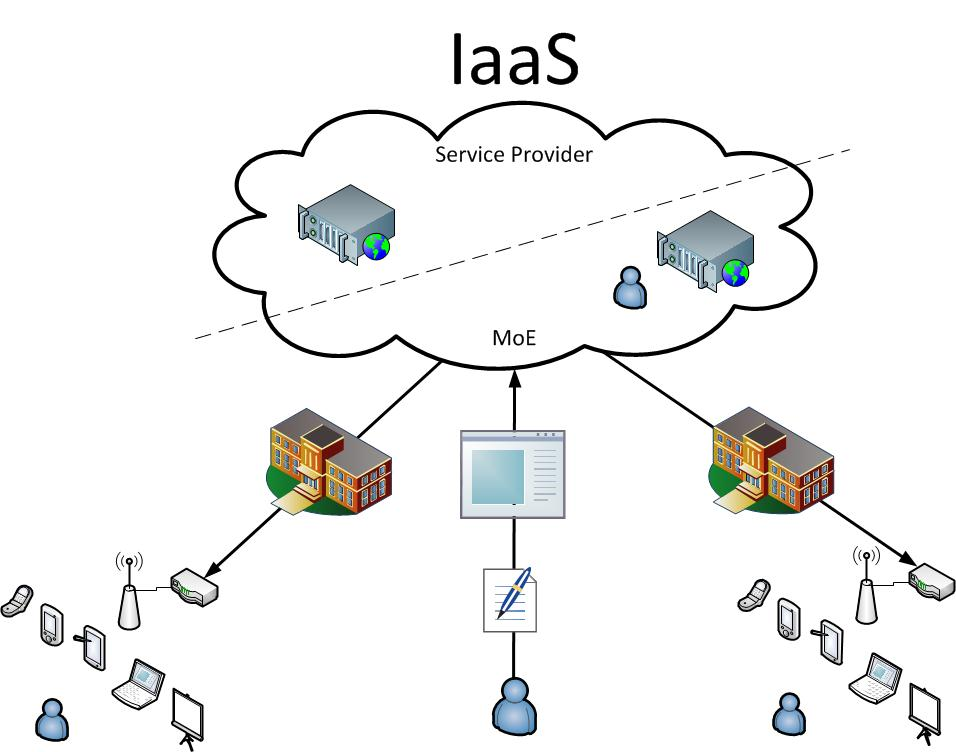
\includegraphics[width=0.7\textwidth]{IaaS.jpg}
	    \caption{ Υπηρεσίες IaaS cloud computing.  }
	    \label{fig:iaas}
	\end{figure}
		
		\subsubsection{PaaS}
	
		Η πλατφόρμα σαν υπηρεσία παρέχει στους πελάτες του υπολογιστικού νέφους όλους τους πόρους και τα εργαλεία που απαιτούνται για να έχουν την δυνατότητα να αναπτύξουν, να διαχειριστούν και να τρέξουν εφαρμογές στο διαδίκτυο χωρίς την πολυπλοκότητα και την ανάγκη εγκατάστασης της υποδομής (λογισμικού) που συνήθως συνδέονται με την ανάπτυξη και την έναρξη μιας εφαρμογής. Οι πλατφόρμες σαν υπηρεσίες προσφέρονται σε δύο διαφορετικές μορφές: είτε σαν δημόσιες cloud υπηρεσίες από τον πάροχο στις οποίες  ο χρήστης  ελέγχει την ανάπτυξη του λογισμικού και τις ρυθμίσεις διαμόρφωσης καθώς ο πάροχος εξασφαλίζει το απαραίτητο υπόβαθρο που χρειάζεται η εφαρμογή, είτε σαν λογισμικό που εγκαθίσταται σε ιδιωτικά κέντρα δεδομένων ή δημόσια υποδομή ως υπηρεσία που διοικείται από εσωτερικά συστήματα πληροφορικής. 
		
		Στο μοντέλο PaaS ο χρήστης δεν ελέγχει την υποκείμενη cloud υποδομή, η οποία συμπεριλαμβάνει το δίκτυο, τους servers, το λειτουργικό σύστημα και τους αποθηκευτικούς χώρους αλλά έχει τον πλήρη έλεγχο στις εγκατεστημένες ή αναπτυγμένες εφαρμογές καθώς και στις ρυθμίσεις των παραμέτρων που γίνονται στο περιβάλλον. Το μοντέλο PaaS βασίζεται σε χρήση της HTML ή Javascript. Υπάρχουν διάφοροι τύποι του μοντέλου PaaS, δημόσιοι, ιδιωτικοί και υβριδικοί. Σε αυτού του τύπου το μοντέλο παροχής υπηρεσιών cloud απαιτούνται δύο επίπεδα προστασίας για την διασφάλιση της ασφάλειας της ιδιωτικής ζωής. Στο χαμηλότερο επίπεδο του συστήματος, ο πάροχος cloud μπορεί να παρέχει βασικούς μηχανισμούς ασφαλείας, όπως end-to-end κρυπτογράφηση, έλεγχο ταυτότητας και εξουσιοδότηση. Στο υψηλότερο επίπεδο, ο  χρήστης των υπηρεσιών cloud χρειάζεται να καθορίσει τις πολιτικές ελέγχου της πρόσβασης στην εφαρμογή.\cite{Kanagaraj2011}
		
		Στα κύρια πλεονεκτήματα του μοντέλου PaaS είναι συγκαταλέγεται αρχικά το γεγονός ότι επιτρέπει τον προγραμματισμό υψηλού επιπέδου με υπερβολικά επίπεδα πολυπλοκότητας. Επιπροσθέτως καθιστά την ολική ανάπτυξη μίας εφαρμογής πιο αποτελεσματική, εφόσον έχει ενσωματωμένη δομή και την συντήρηση - βελτίωση της πιο εύκολη. Ένα άλλο σημαντικό πλεονέκτημα αποτελεί η υψηλή διαθεσιμότητα, η ελαστικότητα και η ευελιξία που προσφέρει με τις ικανότητες πλήρους αυτοδιαχείρισης και αυτό-κλιμάκωσης της υποδομής και της πλατφόρμας εφαρμογών. Βασικό μειονέκτημα αποτελεί η έλλειψη δια-λειτουργικότητας και μεταφοράς της εφαρμογής από τον έναν πάροχο στον άλλον. 

	\begin{figure}[h]
	    \centering
	    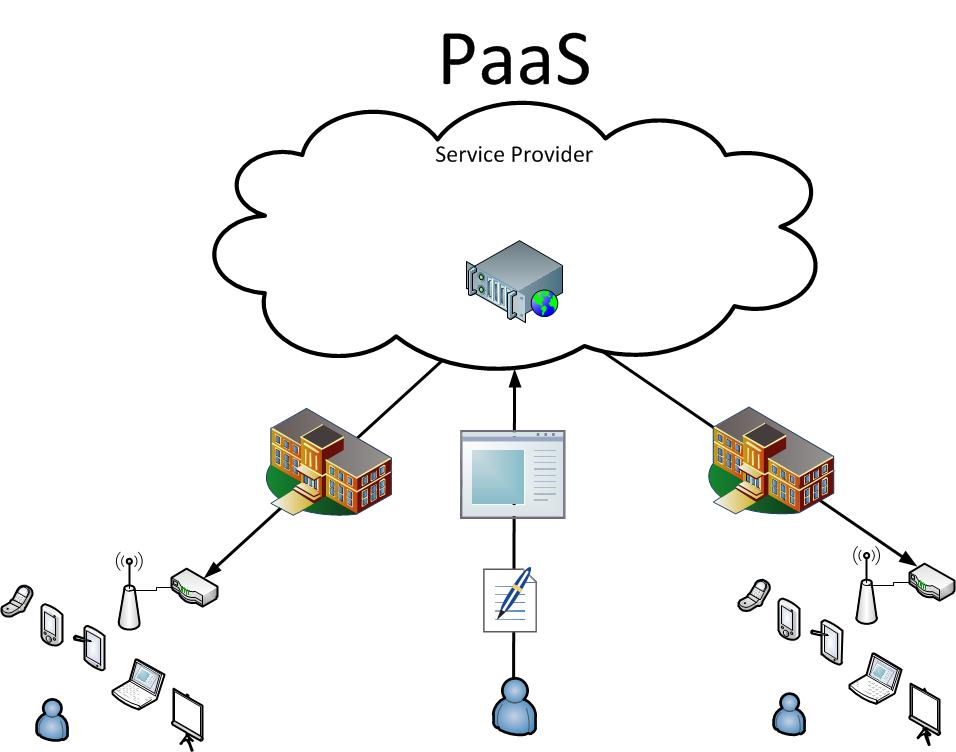
\includegraphics[width=0.7\textwidth]{PaaS.jpg}
	    \caption{Υπηρεσίες PaaS cloud computing.  }
	    \label{fig:paas}
	\end{figure}

		\subsubsection{SaaS}
	 
	Το λογισμικό σαν υπηρεσία είναι ένα μοντέλο ανάπτυξης λογισμικού σύμφωνα με το οποίο παρέχονται κατόπιν ζήτησης στον χρήστη εφαρμογές και υπολογιστικοί πόροι. Ουσιαστικά, είναι όλες οι υπηρεσίες του cloud στις οποίες οι χρήστες είναι σε θέση να αποκτήσουν πρόσβαση σε εφαρμογές μέσω σύνδεσης στο Internet. Οι εφαρμογές αυτές βρίσκονται στο cloud και μπορούν να χρησιμοποιηθούν για ένα ευρύ φάσμα δραστηριοτήτων, τόσο από εταιρείες όσο και από άτομα. Η χρήση των εφαρμογών αυτών αποτελεί περισσότερο ενοικίαση λογισμικού παρά αγορά του. Με την παραδοσιακές εφαρμογές λογισμικού αρχικά αγοράζεται το λογισμικό ως πακέτο, εγκαθίσταται σε έναν υπολογιστή και συνήθως οι σχετικές άδειες περιορίζουν τον αριθμό των χρηστών και των συσκευών όπου μπορεί να αναπτυχθεί το λογισμικό. Εν αντιθέσει, οι χρήστες των υπηρεσιών SaaS εγγράφονται στο λογισμικό, χωρίς να το αγοράσουν, συνήθως σε μηνιαία βάση. 
	
	Οι περισσότεροι χρήστες χρησιμοποιούν έναν λεπτό πελάτη (thin client) για να αποκτήσουν πρόσβαση στις υπηρεσίες SaaS. Οι υπηρεσίες SaaS Οι εταιρικοί χρήστες χρησιμοποιούν τις εφαρμογές που παρέχει ο πάροχος cloud για ανάγκες όπως λογισμικό γραφείου, λογισμικό ανταλλαγής μηνυμάτων,  λογισμικό λογιστικής και τιμολόγησης, λογισμικό για παρακολούθηση των επιδόσεων, λογισμικό διαχείρισης των επιχειρησιακών σχέσεων και πολλά άλλα. 
	
	Βασικά πλεονεκτήματα τους είναι η ευελιξία και η επεκτασιμότητα που προσφέρουν, καθώς οι χρήστες δεν χρειάζεται να αγοράσουν άλλο λογισμικό ή άλλον server, απλά ενεργοποιούν νέες προσφορές του μοντέλου SaaS. Πολύ σημαντικό είναι επίσης η υψηλή ποιότητα των υπηρεσιών η υψηλή σταθερότητα και το γεγονός ότι απαιτείται ελάχιστη συντήρηση. Υπάρχει μεγάλο χρονικό κέρδος, καθώς στις υπηρεσίες SaaS το λογισμικό είναι ήδη εγκατεστημένο και ρυθμισμένο, και η εφαρμογή μπορεί να διατεθεί κατευθείαν στον χρήστη έτοιμη για χρήση. Η πολιτική κοστολόγησης της χρήσης των υπηρεσιών είναι ιδιαίτερα συμφέρουσα συγκριτικά με την αγορά του λογισμικού και πολλές φορές επιτρέπει την χρήση εφαρμογών που σε άλλη περίπτωση θα ήταν απαγορευμένες, λόγω ιδιαίτερα υψηλού κόστους. Θεωρείται αξιόπιστη λύση ασφαλείας , καθώς υιοθετεί SSL (Secure Socket Layer) στις υπηρεσίες του με αποτέλεσμα τα δεδομένα να μεταδίδονται από και προς τον χρήστη με ασφάλεια. Βασικό μειονέκτημα αποτελεί το γεγονός ότι παρέχει πρόσβαση βασισμένη σε ένα δίκτυο που αποτελείται από εμπορικές εφαρμογές με αποτέλεσμα να μην μπορεί πάντα κάποιος να βρει το λογισμικό που ψάχνει διαθέσιμο στο SaaS. 
	
		\begin{figure}[h]
	    \centering
	    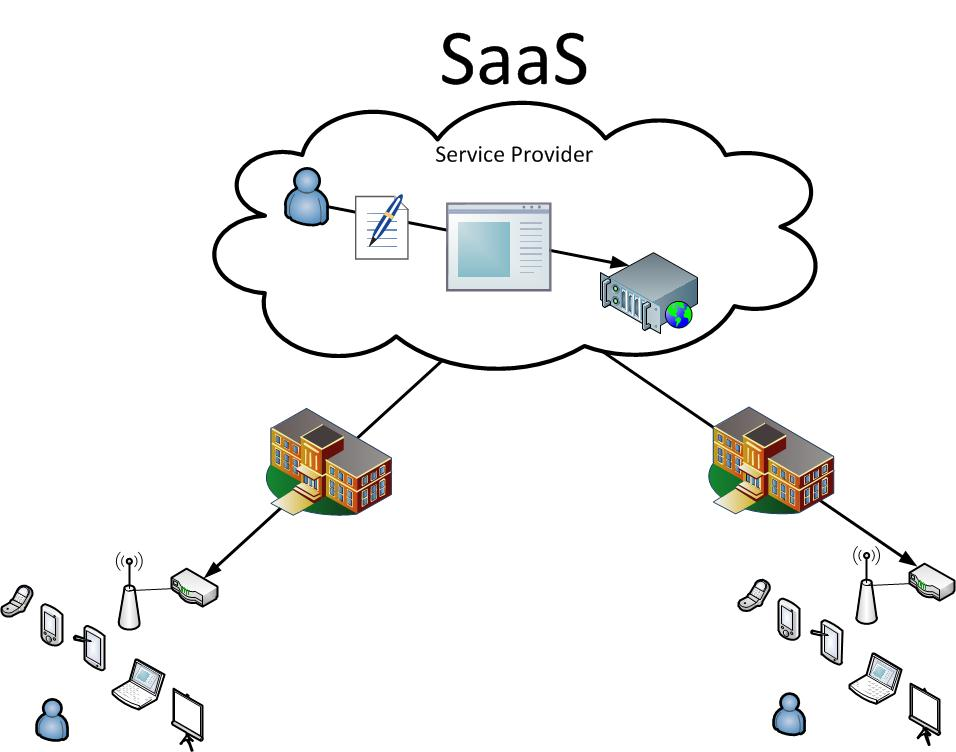
\includegraphics[width=0.7\textwidth]{SaaS.jpg}
	    \caption{Υπηρεσίες SaaS cloud computing.}
	    \label{fig:saas}
	\end{figure}
	
		\subsubsection{BaaS}
 
	
	Η υπηρεσία BaaS είναι ένα μοντέλο που παρέχει στους προγραμματιστές διαδικτυακών εφαρμογών και εφαρμογών για κινητά τηλέφωνα έναν τρόπο για να συνδέουν τις εφαρμογές τους με τον χώρο αποθήκευσης για backend στο cloud και με τα APIs που χρησιμοποιούνται σε backend εφαρμογές.  Επιπλέον παρέχει υπηρεσίες όπως η διαχείριση χρηστών, ειδοποιήσεις (push notifications), κώδικα server και σύνδεση με υπηρεσίες κοινωνικών δικτύων.  Όλες αυτές οι υπηρεσίες παρέχονται μέσω της χρήσης εργαλείων ανάπτυξης λογισμικού (SDKs) και έχουν την δική τους διεπαφή προγραμματισμού εφαρμογών (APIs), που τους επιτρέπει να ενσωματωθούν στις εφαρμογές χωρίς ιδιαίτερο κόπο. Η παροχή ενός σταθερού τρόπου για την διαχείριση των backend δεδομένων συνεπάγεται το γεγονός ότι οι προγραμματιστές δεν χρειάζεται να αναπτύξουν κώδικα backend για κάθε υπηρεσία που η εφαρμογή τους χρησιμοποιεί ή έχει πρόσβαση.

	Ένα από τα κύρια πλεονεκτήματα της χρήσης υπηρεσιών BaaS είναι η τεράστια μείωση του χρόνου ολοκλήρωσης και διατήρησης της εφαρμογής , σε ποσοστό μέχρι και 60\%. Επιπλέον ευνοείται η κλιμάκωση, καθώς το BaaS παρέχει ένα συγκεκριμένο backend το οποίο διαμορφώνει κάποιος εύκολα με βάση τις ανάγκες της εφαρμογής. Η ανάλυση της εφαρμογής γίνεται πιο αποδοτική, καθώς το BaaS διαχειρίζεται όλη την "κίνηση" που γίνεται μέσα στην εφαρμογή και αναλύει τι συμβαίνει σε αυτήν (ποιοι χρήστες είναι πιο ενεργοί, ποιοι είναι πιο εμπλεκόμενοι κ.λ.π. ). Παρά τα πολλά οφέλη του BaaS, είναι επίσης σημαντικό να ληφθεί υπόψιν η κατασκευή του user-interface (UI), διότι αυτό βρίσκεται σε άμεση επικοινωνία με τους τελικούς χρήστες. Ο ρόλος του UI είναι να συνδέεται η εφαρμογή σε οποιοδήποτε άλλο κομμάτι μέρος ή σε αποκλειστικά APIs που συνδέονται στο backend κάτι το οποίο με χρήση των υπηρεσιών BaaS δεν είναι δυνατό πολλές φορές καθώς μια εφαρμογή "κλειδώνεται" στον πάροχο.
	
		\begin{figure}[h]
	    \centering
	    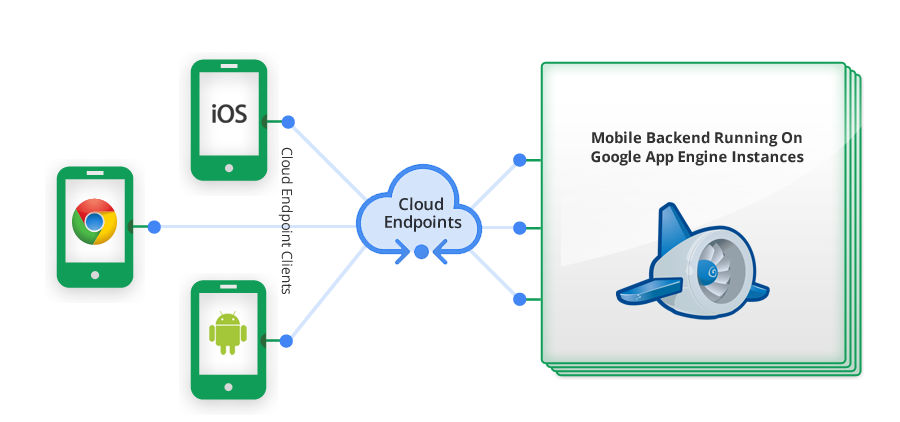
\includegraphics[width=0.7\textwidth]{BaaS.png}
	    \caption{Υπηρεσίες BaaS cloud computing. }
	    \label{fig:baas}
	\end{figure}

	Στην συνέχεια θα αναπτυχθούν τα μοντέλα ανάπτυξης του cloud computing.
	\subsubsection{Public cloud}
	
 
		Το δημόσιο cloud computing είναι ένα μοντέλο μέσω του οποίου οι χρήστες έχουν πρόσβαση στο cloud μέσω διεπαφών που χρησιμοποιούν τα προγράμματα περιήγησης. Ένα cloud καλείται δημόσιο, όταν οι υπηρεσίες του παρέχονται μέσω ενός δημόσιου δικτύου, όπως το διαδίκτυο και είναι ανοιχτές για δημόσια χρήση. Τα δημόσια cloud παρέχουν υπηρεσίες σε πολλούς πελάτες χρησιμοποιώντας την ίδια διαμοιραζόμενη υποδομή.Πολλά δημόσια clouds δεν χρεώνουν τον χρήστη.
		
		 Οι υπηρεσίες SaaS όπως η αποθήκευση στο cloud και οι online εφαρμογές γραφείου είναι οι υπηρεσίες που βρίσκονται κατά κόρον σε δημόσια clouds. Οι υπηρεσίες υποδομής (IaaS) καθώς και οι πλατφόρμες σαν υπηρεσία (PaaS) , κυριώς οι περιπτώσεις του cloud web hosting και των περιβαλλόντων ανάπτυξης αναπτύσσονται εξίσου συχνά και σε δημόσια και σε ιδιωτικά clouds. Τα δημόσια clouds  χρησιμοποιούνται ευρέως σε προσφορές για ιδιώτες οι οποίοι είναι λιγότερο πιθανόν να χρειαστούν το επίπεδο των υποδομών και την ασφάλεια που προσφέρουν τα ιδιωτικά clouds. Ωστόσο, σε πολλές περιπτώσεις οι επιχειρήσεις μπορούν να χρησιμοποιούν δημόσια clouds σεπεριπτώσεις που δεν τίθεται θέμα ευαίσθητων δεδομένων (π.χ. webmai, online συνεργασία) για να κάνουν τις λειτουργίες τους πιο αποτελεσματικά.	\cite{characteristics}

			Τα βασικά πλεονεκτήματα του δημόσιου cloud είναι:
			\begin{itemize}

			\item Απόλυτη επεκτασιμότητα. Το γεγονός ότι οι υπολογιστικοί πόροι στο cloud είναι "ανεξάντλητοι" και γίνονται διαθέσιμοι ανάλογα με τη ζήτηση έχει ως αποτέλεσμα οι εφαρμογές που τρέχουν σε αυτούς να μπορούν να ανταποκριθούν στις διακυμάνσεις της δραστηριότητας.
			
			\item Αποδοτικό. Τα δημόσια clouds συνεπάγονται υψηλότερα επίπεδα υπολογιστικών πόρων με ταυτόχρονα λιγότερο κόστος. Μερικές προτάσεις μαζική αγοράς μπορούν ακόμη και να είναι δωρεάν για τον πελάτη και να στηρίζονται στις διαφημίσεις για τα έσοδα τους (Google).
			
			\item Το μοντέλο πληρωμής ανάλογα με την χρήση. Ο χρήστης είναι σε θέση να αποκτήσει πρόσβαση στους πόρους που χρειάζεται, όποτε θέλει και να πληρώσει μόνο για αυτούς αποφεύγοντας τους περιττούς πόρους.

			\item 	Ευελιξία. Υπάρχει ένας τεράστιος αριθμός των IaaS, PaaS και SaaS υπηρεσιών που διατίθενται στην αγορά, οι οποίες ακολουθούν το μοντέλο του δημόσιου cloud και τις οποίες ο χρήστης μπορεί να προσεγγίσει από οποιαδήποτε συσκευή με χρήση internet. Οι υπηρεσίες αυτές μπορούν να εκπληρώσουν τις περισσότερες υπολογιστικές απαιτήσεις και μπορούν να χρησιμοποιηθούν εξίσου αποτελεσματικά  από ιδιώτες και επιχειρήσεις. 
			
			\item Ανεξαρτησία της τοποθεσίας. Η διαθεσιμότητα των υπηρεσιών του δημόσιου cloud μέσα από το διαδίκτυο εξασφαλίζει ότι οι υπηρεσίες είναι διαθέσιμες όπου και αν βρίσκεται ο χρήστης. Αυτό το γεγονός πολλές φορές είναι ιδιαίτερα χρήσιμο όπως για παράδειγμα σε εταιρίες που δίνεται η δυνατότηα για απομακρυσμένη πρόσβαση σε υποδομές πληροφορικής (σε περίπτωση έκτακτης ανάγκης, κλπ).
			
		\end{itemize}
			
			
	\subsubsection{Private cloud}

	 
	Το ιδιωτικό cloud, είναι ένα μοντέλο το οποίο λειτουργεί αποκλειστικά για έναν οργανισμό, διευθύνεται είτε από τον ίδιο τον οργανισμό είτε από τρίτους και εγκαθίσταται είτε εσωτερικά είτε εξωτερικά. Περιλαμβάνει ένα ξεχωριστό και ασφαλές περιβάλλον με το οποίο μπορούν να αλληλεπιδράσουν οι   χρήστες. Τα ιδιωτικά clouds παρέχουν μεγάλη υπολογιστική ισχύ σαν υπηρεσία χρησιμοποιώντας ένα σύνολο από φυσικούς υπολογιστικούς πόρους, οι οποίοι είναι προσβάσιμοι μόνο από έναν οργανισμό, εξασφαλίζοντας περισσότερο έλεγχο και αυξημένη ασφάλεια. Τα δημόσια clouds περιλαμβάνουν πολλούς πελάτες οι οποίοι έχουν πρόσβαση σε εικονικές υπηρεσίες που αντλούν πόρους από την ίδια ομάδα από servers μέσω δημοσίων δικτύων. Τα ιδιωτικά clouds από την άλλη πλευρά, περιλαμβάνουν την οριοθέτηση ενός cloud για την αποκλειστική χρήση ενός οργανισμού. Παρόλο που χρησιμοποιούνται ξεχωριστοί πόροι, μπορούν να γίνουν προσβάσιμοι μέσω ιδιωτικών γραμμών ή ασφαλών κρυπτογραφημένων συνδέσεων μέσω των δημόσιων δικτύων. 
	
	Τα ιδιωτικά cloud είναι κατάλληλα για περιπτώσεις στις οποίες υπάρχει η ανάγκη αποθήκευσης και επεξεργασίας ιδιωτικών η ευαίσθητων δεδομένων ή η ανάγκη διεξαγωγής ευαίσθητων εργασιών. Για παράδειγμα, μία ιδιωτική cloud υπηρεσία μπορεί να χρησιμοποιηθεί από ένα πληροφοριακό σύστημα με που διαχειρίζεται και αποθηκεύει ευαίσθητα ιατρικά δεδομένα και θέλει να επωφεληθεί από τα πλεονεκτήματα του cloud computing στην επιχειρησιακή υποδομή του. 	Υιοθετεί τις βασικές αρχές ασφαλείας, νομοθεσίας και κανονιστικών απαιτήσεων αφού προσφέρει μεγάλο έλεγχο εγκατάστασης και χρήσης στην επιχείρηση που το χρησιμοποιεί.Το ιδιωτικό μοντέλο cloud μοιάζει  αρκετά με το μοντέλο των  δικτύων τοπικής πρόσβασης (LAN) που χρησιμοποιούταν στο παρελθόν αλλά παρέχει τα επιπλέον πλεονεκτήματα του cloud. Κάποια από τα πλεονεκτήματα του ιδιωτικού cloud είναι:
	
	\begin{itemize}
	
	\item Μεγαλύτερη προστασία και ασφάλεια. Τα δημόσια clouds εφαρμόζουν μηχανισμούς παροχής ασφάλειας, αλλά τα ιδιωτικά clouds με τους αποκλειστικούς φυσικούς πόρους που επιτρέπουν πρόσβαση μόνο σε συνδέσεις που γίνονται μέσω συγκεκριμένου οργανισμού και προσωπικές ασφαλείς γραμμές εξασφαλίζουν ότι υπάρχει πλήρης ασφάλεια και αξιοπιστία.
	
	\item Περισσότερο έλεγχο με αποτέλεσμα περισσότερη ευελιξία. Εφόσον η πρόσβαση στους πόρους γίνεται μόνο από έναν οργανισμό, αυτός ο οργανισμός έχει την ικανότητα να ρυθμίσει και να διαχειριστεί το cloud όπως επιθυμεί ώστε να επιτευχθεί το κατάλληλο δίκτυο. 
	
	\item Βελτίωση  της σχέσης κόστους και ενεργειακής απόδοσης. Η εφαρμογή ενός ιδιωτικού μοντέλου cloud μπορεί να συντελέσει στην καλύτερη κατανομή των πόρων σε έναν οργανισμό, εξασφαλίζοντας ότι η διαθεσιμότητα των πόρων ανταποκρίνεται άμεσα και ευέλικτα ανάλογα με την ζήτηση τους. Παρόλο που είναι πιο ακριβά σε σχέση με τα δημόσια clouds, κάνουν πιο αποτελεσματική χρήση των υπολογιστικών πόρων σε σχέση με τα παραδοσιακά τοπικά δίκτυα (LANs), καθώς ελαχιστοποιείται η επένδυση σε αχρησιμοποίητη παραγωγική ικανότητα. 
	
	\item Βελτιωμένη αξιοπιστία. Ακόμα και αν οι πόροι (servers, δίκτυα, κ.λ.π.) φιλοξενούνται εσωτερικά στον πελάτη, η δημιουργία εικονικών περιβάλλοντων λειτουργικού συνεπάγεται ότι το δίκτυο είναι πιο ανθεκτικό σε επιμέρους αστοχίες από ότι η φυσική υποδομή. 

	\end{itemize}
	
		
		\subsubsection{Community cloud}
		\subsubsection{Hybrid cloud}
		
		\subsubsection{NodeJs}
		\subsubsection{Cloud και ασφάλεια Ιατρικών δεδομένων?}
	\subsection{Βάση Δεδομένων}
	Στον τομέα της επιστήμης των υπολογιστών όταν αναφερόμαστε στον όρο NoSQL (Not Only SQL), μιλάμε για ένα ευρύ φάσμα συστημάτων διαχείρισης βάσεων δεδομένων τα οποία παρέχουν ένα μηχανισμό προς αποθήκευση και ανάκτηση δεδομένων διαφορετικό από αυτό του σχεσιακού μοντέλου των κλασσικών RDBMS (Relational database management system). Τα συστήματα NoSQL ξεφεύγουν από την παραδοσιακή χρήση πινάκων για την οργάνωση των δεδομένων και χρησιμοποιούν διαφορετικές δομές οργάνωσης όπως αυτή του κλειδιού-τιμής. Επιπροσθέτως η επεξεργασίά αυτών των δεδομένων δεν γίνεται με χρήση ερωτημάτων SQL όπως έχουμε συνηθίσει. Λόγω των εγγενών διαφορών μεταξύ των δύο αυτών συστημάτων, κάποιες λειτουργίες είναι ταχύτερες στα συστήματα NoSQL ενώ κάποιες άλλες στα συστήματα σχεσιακών βάσεων δεδομένων.
	
	Η χρήση των βάσεων δεδομένων τύπου NoSQL έχει γνωρίσει ραγδαία αύξηση τα τελευταία χρόνια σε εφαρμογές big data καθω και σε εφαρμογές πραγματικού χρόνου. Αποκαλούνται με τον όρο Not Only SQL για να δοθεί έμφαση στο γεγονός ότι οι δύο τεχνολογίες δεν είναι αμοιβαία αποκλειόμενες. Έχουν την δυνατότητα να συνυπάρχουν, κρατώντας τα δυνατά σημεία της κάθε μιας, προσφέροντας σε διαφορετικές καταστάσεις διαφορετικές υπηρεσίες. Οι βάσεις δεδομένων τύπου NoSQL χρησιμοποιούνται από τις εταιρείες κολοσσούς του τεχνολογικού τομέα όπως το Facebook, Amazon, Google, LinkedIn.
	
%  ΑΝ ΤΟ ΒΑΛΕΙΣ ΒΡΕΣ ΠΗΓΕΣ ΚΑΙ ΔΙΑΒΑΣΕ ΛΕΠΤΟΜΕΡΕΙΕΣ	 Πολλές NoSQL αποθηκεύσεις θέτουν σε κίνδυνο τη συνοχή (με την έννοια του θεωρήματος CAP) για χάρη της διαθεσιμότητας και της τμηματικής ανεκτικότητας. Εμπόδια για την ευρύτερη υιοθέτηση των NoSQL αποθηκεύσεων αποτελούν η χρήση χαμηλού επιπέδου γλωσσών ερωτημάτων, η έλλειψη τυποποιημένων διεπαφών και οι τεράστιες επενδύσεις στην υπάρχουσα SQL. Οι περισσότερες NoSQL αποθηκεύσεις στερούνται πραγματικών ACID συναλλαγών, παρόλο που μερικά πρόσφατα συστήματα, όπως το FairCom c-treeACE, το Google Spanner και το FoundationDB, τις έχουν κάνει βασικές στο σχεδιασμό τους
		\subsubsection{Σχετικά με NoSql}
			NoSql vs Relation DB - βρες κάτι και για medical με nosql. Γιατί NoSql. Γιατί MongoDb.
		\subsubsection{Schema}

\section{Front-End}
	\subsection{Αρχιτεκτονική}
		\subsubsection{MVC αρχιτεκτονικό πρότυπο}\label{sssection:mvc}

		Το σχεδιαστικό μοτίβο Model View Controller (MVC) είναι ένα αρχιτεκτονικό πρότυπο που χρησιμοποιείται στην τεχνολογία λογισμικού και συνήθως στην υλοποίηση web εφαρμογών. Χωρίζει την εφαρμογή σε τρία διασυνδεδεμένα μέρη, με σκοπό τον πλήρη διαχωρισμό της εσωτερικής αναπαράστασης  της πληροφορίας στο σύστημα από τους τρόπους παρουσίασης της πληροφορίας στον χρήστη. Το MVC αποτελείται από τρία στοιχεία: α) Model, β) View, γ) Controller.
		\begin{itemize} 
		\item\textbf{Model:} Το model είναι το κομμάτι της εφαρμογής που αναπαριστά την πληροφορία, δηλαδή τα δεδομένα που χρησιμοποιεί η εφαρμογή και επιβάλλει τις ενέργειες και τους περιορισμούς πάνω σε αυτά.  Στο model τοποθετούμε τις λειτουργίες της εφαρμογής που σχετίζονται με την πρόσβαση στη βάση δεδομένων. Οι λειτουργίες αυτές είναι συναρτήσεις με τις οποίες διαχειριζόμαστε αποτελεσματικά τα δεδομένα που λαμβάνουμε από τη βάση.  Το μοντέλο ανταποκρίνεται σε ερωτήματα από το view καθώς και σε οδηγίες από τον controller για να πραγματοποιήσει ενημερώσεις.
		\item\textbf{View:} Αντιστοιχεί στην γραφική παρουσίαση των δεδομένων του model στο interface του χρήστη. Ο controller, είναι αυτός ο οποίος αποφασίζει πότε θα παρουσιαστούν τα δεδομένα ενώ το view καθορίζει τον τρόπο με τον οποίο θα παρουσιαστούν τα δεδομένα στον χρήστη. Το επίπεδο view θα πρέπει να προσαρμόζεται στις αλλαγές του επιπέδου του model, για αυτό και τα views θα πρέπει να επικεντρώνονται μόνο στην εμφάνιση δεδομένων και να μην εμπλέκονται με την επιχειρηματική λογική του model.
		\item\textbf{Controller:} Ο controller είναι αυτός που παίρνει αποφάσεις, δηλαδή διαχειρίζεται τη σύνδεση των δεδομένων του model με τη λογική του προγράμματος και καθορίζει ποια από τα δεδομένα του model θα παρουσιαστούν από το view στο interface του χρήστη. Ο controller ενημερώνει το view κάθε φορά που αλλάζει το model. Επιπλέον προσθέτει event listeners στο view και ενημερώνει το model όταν ο χρήστης αλληλεπιδρά με το view.
	 \end{itemize}		
	 \begin{figure}[h]
	    \centering
	    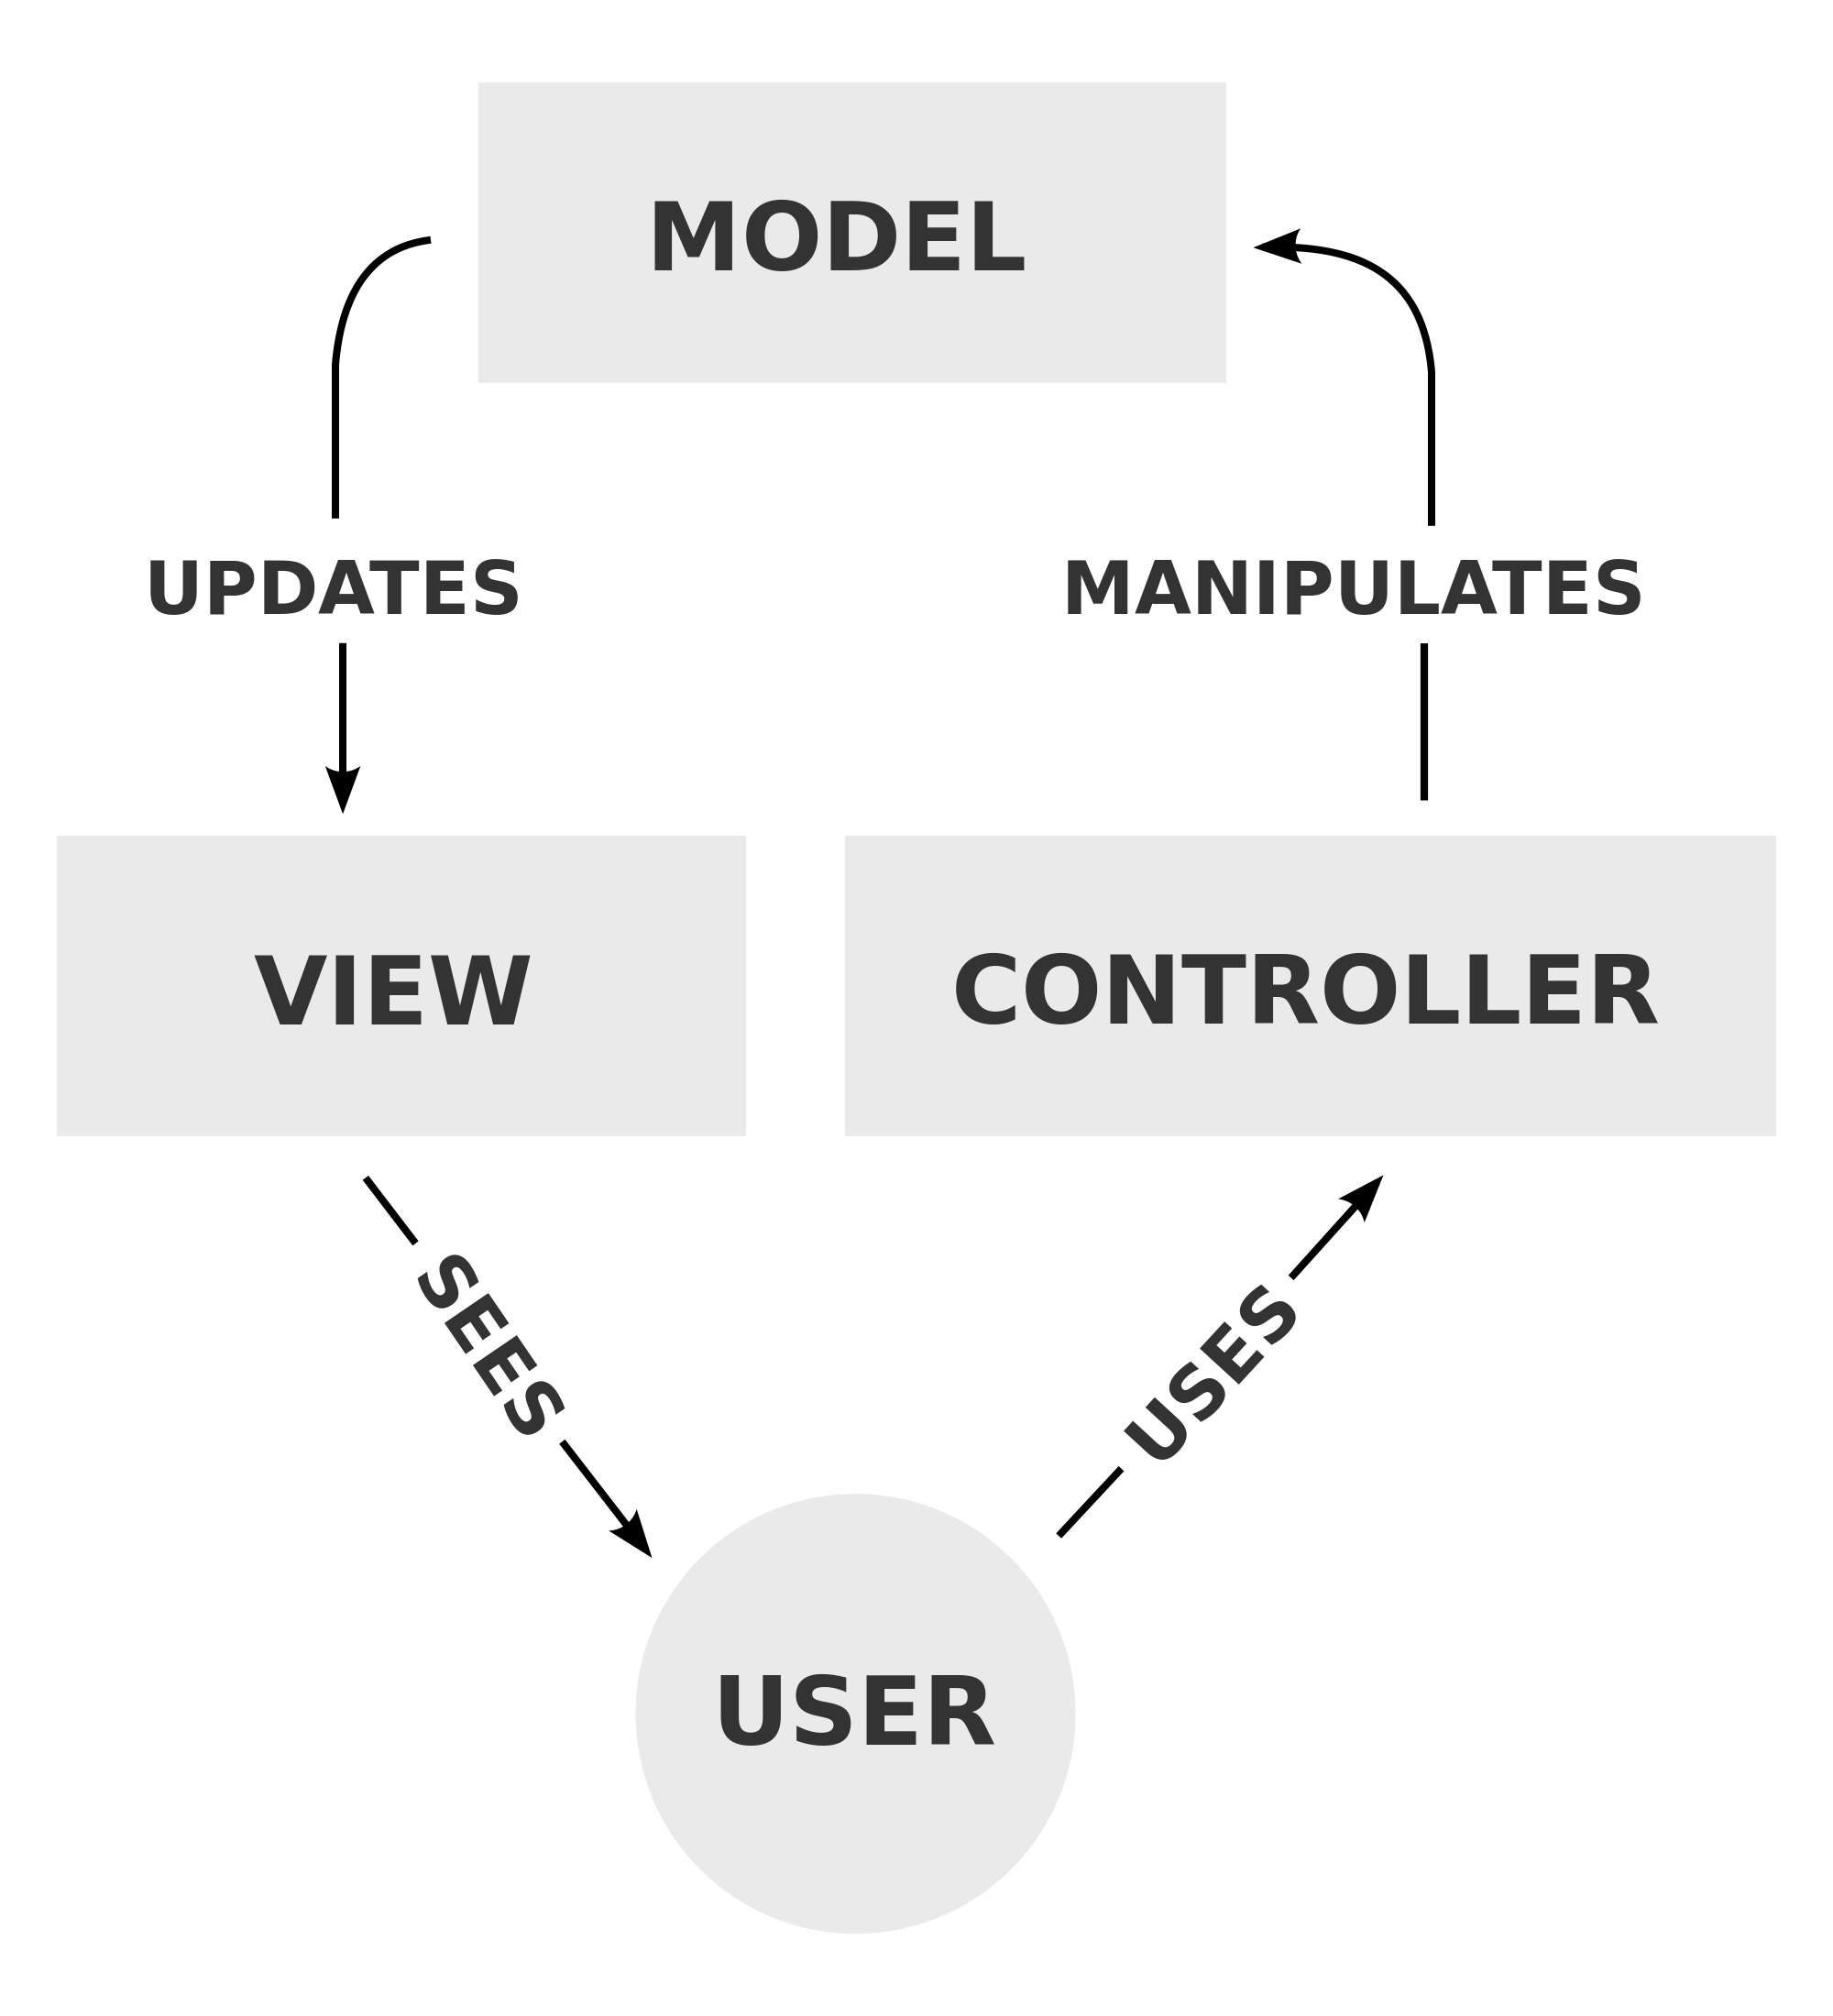
\includegraphics[width=0.7\textwidth]{mvcpattern.png}
	    \caption{Αρχιτεκτονική MVC.}
	    \label{fig:mvc_pattern}
	\end{figure}
		
		
		Η  χρήση της αρχιτεκτονικής MVC κατά την δημιουργία μίας εφαρμογής μας προσφέρει τα εξής βασικά πλεονεκτήματα:
		\begin{itemize}
		\item Διαχωρισμός των προβλημάτων (Separation of Concerns). Ουσιαστικά δημιουργείται μία εφαρμογή η οποία έχει τρία επίπεδα(models, views, controllers) και το κάθε επίπεδο επιτελεί ξεχωριστό έργο και ταυτόχρονα συνεργάζεται με τα άλλα επίπεδα. Στην σωστή υλοποίηση πρέπει τα τρία επίπεδα να είναι πλήρως καθορισμένα και να μην συμπλέκονται. Ο διαχωρισμός αυτός, επιτρέπει την επαναχρησιμοποίηση της επιχειρηματικής λογικής σε διάφορες εφαρμογές και την ανάπτυξη πολλαπλών user interfaces χωρίς να προβληματιζόμαστε από τον κώδικα που διαχειρίζεται την βάση.
		\item \textbf{Επεκτασιμότητα (Scaleability)}. Είναι η δυνατότητα που διαθέτει μία εφαρμογή , να μπορούμε μελλοντικά να προσθέσουμε λειτουργίες σε αυτή ή να αλλάξουμε κάποιες από τις ήδη υπάρχουσες λειτουργίες με σκοπό να επιτύχουμε διαφορετικά αποτελέσματα. 
		\item \textbf{Ελεγξιμότητα (Testability)}. Οι MVC εφαρμογές έχουν την δυνατότητα να είναι πιο εύκολα ελέγξιμες και με τον τρόπο αυτό συντηρούνται πιο εύκολα.  Εφόσον τα συστατικά της αρχιτεκτονικής είναι διακριτά είναι πιο εύκολο να γράφουμε κώδικα που να τεστάρει ξεχωριστά το κάθε κομμάτι, γρήγορα και αποτελεσματικά.
		\item \textbf{Παράλληλη ανάπτυξη από διαφορετικές ομάδες}. Οι προγραμματιστές επιχειρηματικής λογικής  μπορούν να δημιουργούν τις κλάσεις, ενώ οι προγραμματιστές του user interface μπορούν να σχεδιάζουν ταυτόχρονα τις οθόνες. Επίσης μπορούν να γίνονται ενημερώσεις και αλλαγές στο user interface χωρίς να επιβραδύνεται η διαδικασία του business logic.
		\end{itemize}
		
	\subsubsection{MVP αρχιτεκτονικό πρότυπο}
	Το αρχιτεκτονικό πρότυπο Model View Presenter (MVP) αποτελεί ένα παράγωγο αρχιτεκτονικό πρότυπο του MVC \cite{mvpPotel}, το οποίο είναι πολύ δημοφιλές στην ανάπτυξη εφαρμογών για το λειτουργικό σύστημα Android. Στην θεωρία τουλάχιστον, οι εφαρμογές Android είναι στημένες με την λογική του MVC \cite{androidArchAnalysis} όπως περιγράφηκε στην ενότητα \ref{sssection:mvc}, με το Activity ή το Fragment να αποτελεί τον controller και τα xml layouts τα views. Στην πράξη όμως καταλήγει η πλειονότητα του view logic να βρίσκεται στο Activity το οποίο το μετατρέπει σε δομή model-view όπως φαίνεται στο σχήμα \ref{fig:model_view}, κάτι το οποίο σε καμία περίπτωση δεν είναι το επιθυμητό. Στόχος λοιπόν του MVP είναι να λύσει ακριβώς αυτό το πρόβλημα και να πετύχει πλήρη διαχωρισμό μεταξύ του view και του view logic όπως βλέπουμε στο σχήμα \ref{fig:mvp_pattern}.
		
	 \begin{figure}[h]
	    \centering
	    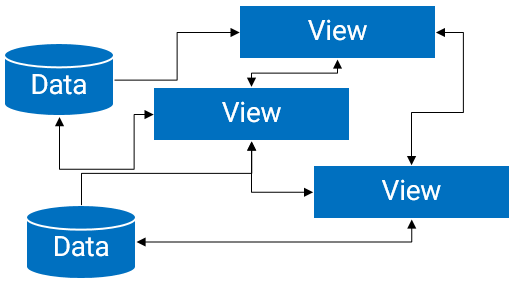
\includegraphics[width=0.7\textwidth]{model_view.png}
	    \caption{Android Model-View αρχιτεκτονικό πρότυπο}
	    \label{fig:model_view}
	\end{figure}
	
	\begin{figure}[h]
	    \centering
	    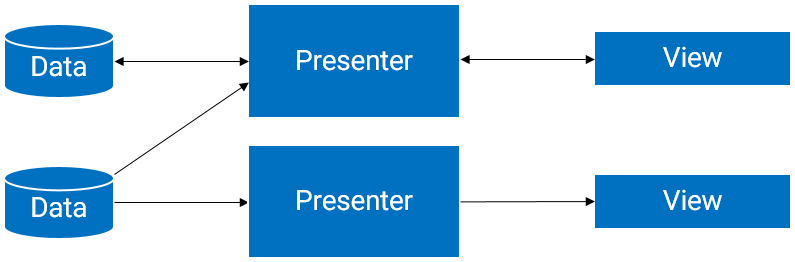
\includegraphics[width=0.7\textwidth]{mvp_pattern.png}
	    \caption{Android MVP αρχιτεκτονικό πρότυπο}
	    \label{fig:mvp_pattern}
	\end{figure}
	
	Πλεονεκτήματα και λόγοι χρήσης του αρχιτεκτονικού προτύπου Model View Presenter\cite{androidHacks}:
	\begin{itemize}
		\item \textbf{Επεκτασιμότητα} η οποία επιτυγχάνεται μέσω του πλήρη διαχωρισμού μεταξύ της εμφάνισης (view) και της λογικής της εμφάνισης (view logic). 
		\item \textbf{Ευκολία Testing} του κάθε στρώματος (layer) της εφαρμογής αφού έχουμε πετύχει σαφή διαχωρισμό μεταξύ τους. Εν γένει η χρήση του μοτίβου MVP προάγει το test driven development της εφαρμογής με όλα τα πλεονεκτήματα που συνεπάγεται η εν λόγω τεχνική ανάπτυξης.
	\end{itemize}
	
	Το αρχιτεκτονικό πρότυπο MVP όπως δηλώνει και το όνομα του αποτελείται από τα παρακάτω τρία στοιχεία α) Model β) View γ) Presenter :
	\begin{itemize}
		\item \textbf{Model: } Το model στο αρχιτεκτονικό πρότυπο MVP επιτελεί της ίδιες λειτουργίες με αυτές στο MVC όπως περιγράφηκαν παραπάνω στην ενότητα \ref{sssection:mvc}.
		\item \textbf{View: } Το view υλοποιείται συνήθως μέσω κάποιου Activity ή Fragment (εξαρτάται από την συγκεκριμένη αρχιτεκτονική της εφαρμογής), και περιέχει αναφορά στον presenter ο οποίος το χειρίζεται. H εν λόγω αναφορά πραγματοποιείται με χρήση του σχεδιαστικού μοτίβου dependency injection και ιδανικά με χρήση του Dagger. Κάθε φορά που ο χρήστης αλληλεπιδρά με κάποια λειτουργία (π.χ κουμπί) του view, καλείται η αντίστοιχη συνάρτηση του presenter ο οποίος επικοινωνεί με το model και λέει εν τέλει στο view τι θα εμφανίσει.
		\item \textbf{Presenter: } Ο Presenter είναι λειτουργεί ως το ενδιάμεσο στάδιο - ενορχηστρωτής μεταξύ του view και του model. Είναι υπεύθυνος για την απόκτηση των δεδομένων από το model και την παρουσίαση τους στο view, αλλά σε αντίθεση με την κλασσική αρχιτεκτονική MVC είναι υπεύθυνος για τις αλλαγές που γίνονται στο view όταν ο χρήστης αλληλεπιδρά μαζί του.
	\end{itemize}
	
	Για να αποσαφηνιστεί πλήρως η λειτουργία του και να γίνει πιο εύκολα κατανοητό στο σχήμα \ref{fig:mvp_workflow} βλέπουμε ένα χαρακτηριστικό παράδειγμα.
	
	\begin{figure}[h]
	    \centering
	    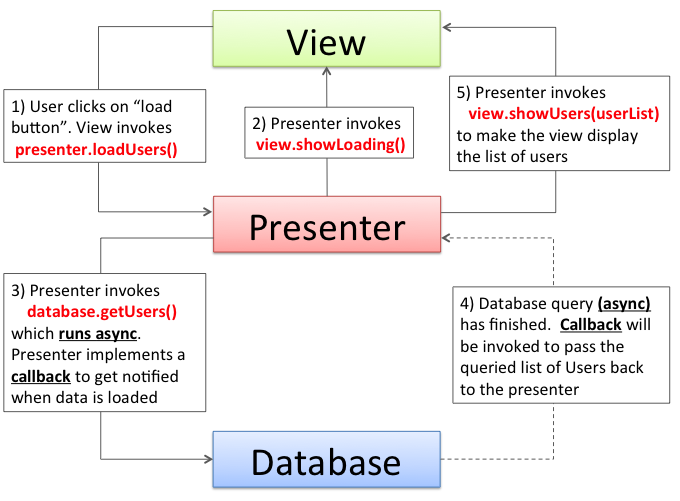
\includegraphics[width=0.7\textwidth]{mvp_workflow.png}
	    \caption{Παράδειγμα MVP σε Android}
	    \label{fig:mvp_workflow}
	\end{figure}

	\subsection{Frameworks}
	
		Το framework, στον προγραμματισμό ηλεκτρονικών υπολογιστών, είναι μια αφηρημένη έννοια με την οποία κοινός κώδικας ο οποίος παρέχει γενικές λειτουργίες, μπορεί να επανεγγραφεί επιλεκτικά ή να εξειδικευτεί μέσω του κώδικα κάποιου χρήστη ώστε να χρησιμοποιηθεί για συγκεκριμένες λειτουργίες. Τα frameworks είναι μια ειδική περίπτωση βιβλιοθηκών λογισμικού που εμπεριέχουν επαναχρησιμοποιήσιμα κομμάτια κώδικα σε μια καλά καθορισμένη διεπαφή προγραμματισμού εφαρμογών (API), που όμως περιέχουν κάποια βασικά χαρακτηριστικά γνωρίσματα που τα διαφοροποιούν από τις κανονικές βιβλιοθήκες. Κάποια από τα γνωρίσματα αυτά είναι: αντιστροφή του ελέγχου (η ροή του προγράμματος υπαγορεύεται από το framework και όχι από αυτόν που το χρησιμοποιεί), προκαθορισμένη συμπεριφορά, επεκτασιμότητα (μπορεί να επεκταθεί από το χρήστη συνήθως με επανεγγραφή  ή εξειδίκευση του κώδικα ώστε να εκτελούνται συγκεκριμένες λειτουργίες. \cite{Framework}

	
		\subsubsection{Express Framework}

		Το Express.js είναι ένα framework του Node.js, σχεδιασμένο για να χτίζει μίας σελίδας, πολλών σελίδων, και hybrid web εφαρμογές. Είναι το προκαθορισμένο framework που χρησιμοποιείται πάνω στο node.js.  Ο δημιουργός του TJ Holowaychuck το περιέγραψε ως ένα "Sinatra inspired server", πράγμα που σημαίνει ότι είναι σχετικά ελάχιστο, με πολλά χαρακτηριστικά διαθέσιμα ως πρόσθετα. Το express είναι το backend της στοίβας MEAN.
		
		\subsubsection{Angular}
		Το AngularJS είναι ένα από τα πιο δημοφιλή ανοιχτού κώδικα JavaScript framework που χρησιμοποιείται για την κατασκευή και τη δομή σύγχρονων διαδικτυακών εφαρμογών, κυρίως εφαρμογών μίας σελίδας. Αναπτύχθηκε από την Google και από μία κοινότητα προγραμματιστών για την αντιμετώπιση των πολλών προκλήσεων που ανέκυψαν κατά την ανάπτυξη των εφαρμογών μίας σελίδας.  Στόχος του είναι να απλοποιήσει τόσο την ανάπτυξη όσο και το testing αυτών των εφαρμογών, παρέχοντας ένα framework για client-side model-View-Controller (MVC) και το model-view-viewmodel (MVVM) αρχιτεκτονικές, μαζί με τα συστατικά που χρησιμοποιούνται συνήθως στις εφαρμογές Διαδικτύου.
	   \\*
			    \textbf{Αρχιτεκτονική}
	 \\*
		Κατά την εκκίνηση της εφαρμογής, το πρόγραμμα περιήγησης φορτώνει το HTML αρχείο και το παρσάρει στο DOM αρχείο, και μαζί με αυτό στο angular.js script. Μόλις το DOM αρχείο έχει φορτωθεί, το AngularJS αναζητά την εντολή ng-app η οποία ορίζει τα όρια της εφαρμογής. Εάν ορίζεται κάποιο module μέσα στην οδηγία, τότε χρησιμοποιείται για να ρυθμιστεί το \$injector, που δημιουργεί τo \$compile service καθώς και το \$ rootScope. Τότε μεταγλωττίζεται το DOM και συνδέεται στο \$ rootScope μετά από το οποίο εκτελούνται οι υπόλοιπες εντολές (αν υπάρχουν). Στο σχήμα \ref{fig:angularjs} φαίνεται ο κύκλος εκκίνησης του AngularJS.
	  \begin{figure}[h]
	    \centering
	    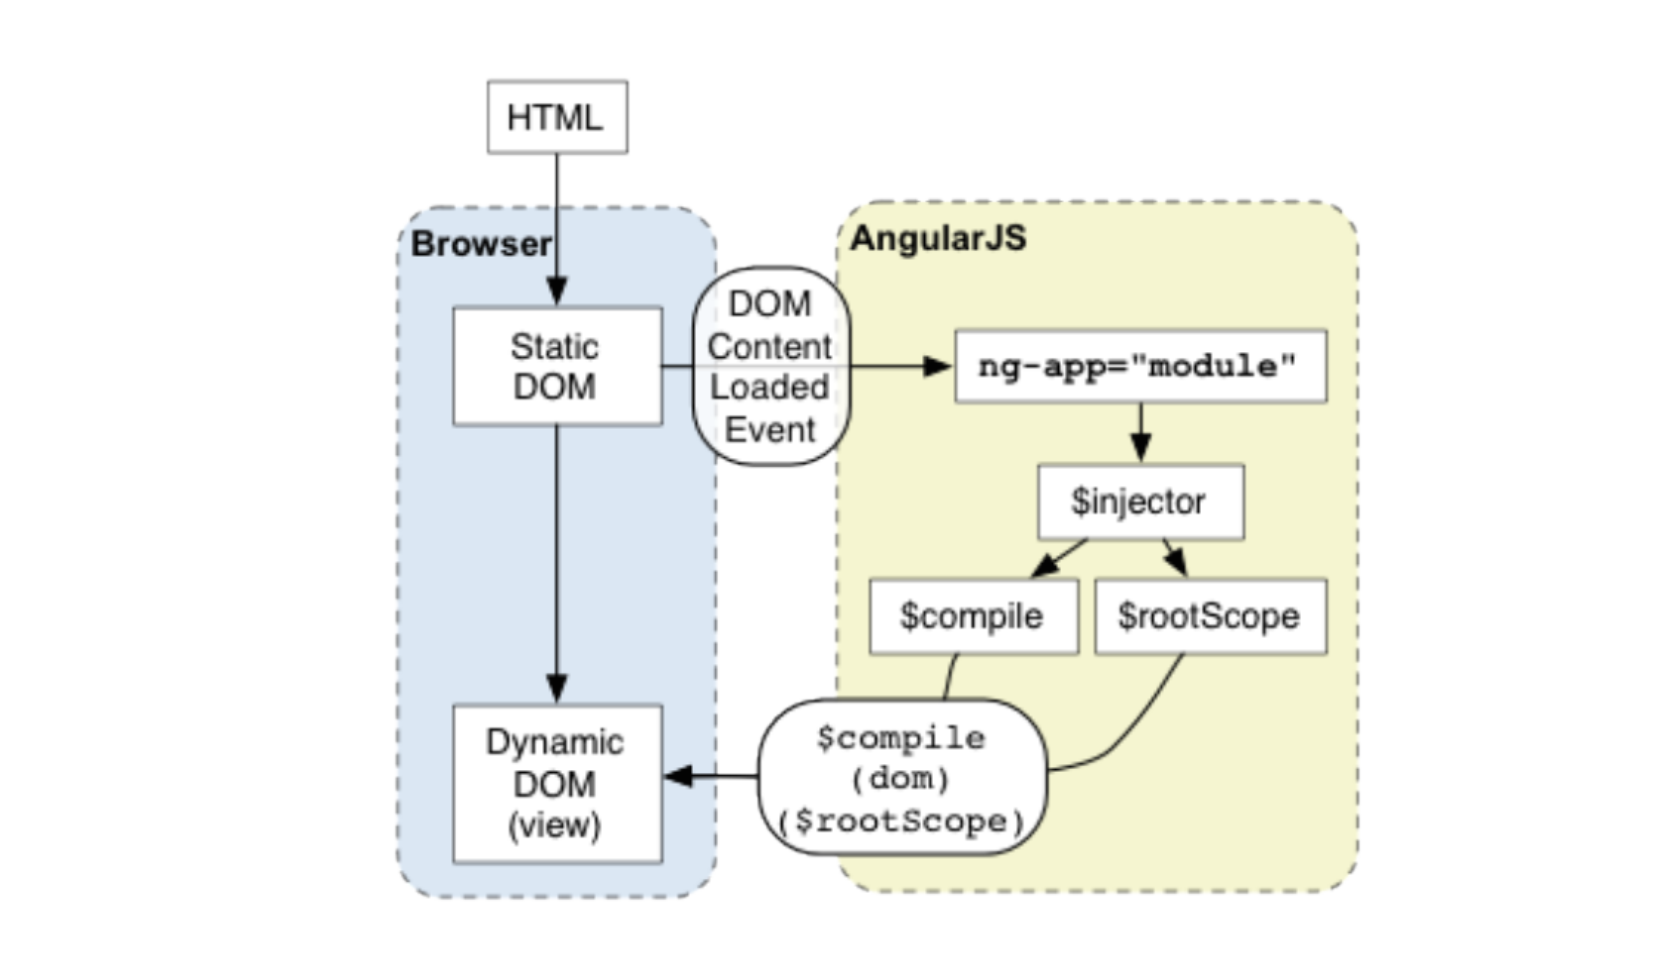
\includegraphics[width=0.7\textwidth]{angularjs.png}
	    \caption{AngularJS κύκλος εκκίνησης.}
	    \label{fig:angularjs}
	\end{figure}

	Κάποια από τα βασικά χαρακτηριστικά του AngularJS είναι:
	\begin{itemize}
	\item Two Way Data-binding. Αυτό πρακτικά σημαίνει ότι όταν αλλάζει το model αλλάζει και το view, και όταν αλλάζει το  view αλλάζει και το model.  Το Two Way Data-binding εξηγείται καλύτερα με ένα παράδειγμα: 
	
	
	\lstinputlisting[language=Html]{two_way_data_binding.html}

	Αν ο χρήστης αλλάζει κάποια τιμή του model μέσω εισόδου στο view, τότε το AngularJs αποθηκεύει την τιμή
αυτή σε μια μεταβλητή. Το στοιχείο h1 στην συνέχεια ενημερώνεται αυτόματα ώστε να αντικατοπτρίζονται οι αλλαγές στην τιμή της μεταβλητής του model. Το view ενημερώνεται ακόμα και αν η μεταβλητή αλλάξει χειροκίνητα με χρήση JavaScript.\cite{angular}

	\item  HTML Templates. Ενώ άλλα JavaScript frameworks χρησιμοποιούν ένα template system που βασίζεται στην HTML με ειδική σήμανση το οποίο μπορεί να είναι δυσκολεύει τους προγραμματιστές, το AngularJS δεν στηρίζεται σε εξωτερικές template engines αλλά χρησιμοποιεί ένα templating σύστημα, που είναι χτισμένη πάνω στην HTML με έξυπνη χρήση των ng- χαρακτηριστικών. Το πρόγραμμα περιήγησης διαβάζει την HTML και "ψάχνει"  ng - directives τα οποία, όταν εκτελεστεί, δεσμεύουν το view στο model.

    \item Dependency Injection. Το dependency injection ενθαρρύνεται πολύ από το AngularJS και είναι ένα από τα συστατικά του, που βελτιώνει σε μεγάλο βαθμό το testability του. Το dependency injection είναι ένα design pattern λογισμικού στο οποίο σε ένα αντικείμενο ορίζονται οι εξαρτήσεις του και δεν τις δημιουργεί μόνο του. Πρόκειται ουσιαστικά για την αφαίρεση των hard-coded εξαρτήσεων κάνοντας δυνατό να αλλάξουν οι εξαρτήσεις όποτε χρειαστεί.
      Ένα παράδειγμα είναι όταν έχεις μία συνάρτηση η οποία παίρνει μία παράμετρο, όπως το ακόλουθο παράδειγμα:
    	
	\lstinputlisting[language=JavaScript]{angular_dependency_injection.js}

Το παραπάνω παράδειγμα είναι εύκολο να το τεστάρουμε, επειδή το στοιχείο που εισάγεται στην συνάρτηση μπορεί να είναι είτε ένα πραγματικό αντικείμενο ή ένα αντικείμενο για τους σκοπούς των τεστ. Ο διαχωρισμός σε μικρότερα πιο εύκολα ελέγξιμα συστατικά μπορεί να βοηθήσει πολύ στην ανίχνευση των σφαλμάτων.

    \item Deep Linking. Σε μια εφαρμογή μίας σελίδας είναι σημαντικό να διατηρείται η κατάσταση της εφαρμογής στο url, έτσι ώστε οι χρήστες είναι σε θέση να βάλουν κάποιο σελιδοδείκτη ή να μοιραστούν κάποιον σύνδεσμο σε διάφορες καταστάσεις της εφαρμογής.Το AngularJS χρησιμοποιεί το HTML5 history API  μαζί με ένα (\#!) εφεδρικό για παλαιότερα προγράμματα περιήγησης. Η λειτουργία αυτή είναι εξαιρετικά ισχυρή στη σύγχρονη εποχή των κοινωνικών δικτύων και του sharing.

	\item Directives. Τα directives είναι κάτι μοναδικό στο AngularJS και επιτρέπουν την επέκταση της λειτουργικότητας της HTML. Ενώ το AngularJS έχει μια συλλογή από προκαθορισμένα directives, μπορεί να επεκταθεί με συγκεκριμένες λειτουργικότητες σε σημείο που να επιτρέπει στον χρήστη να δημιουργήσει το δικό του DSL (Domain specific language). Επίσης επιτρέπει να δημιουργηθούν προσαρμοσμένα στοιχεία DOM, καθώς και χαρακτηριστικά και κλάσεις στα οποία μπορούν να προστεθούν λειτουργικότητες. Το επόμενο παράδειγμα από το επίσημο documentation του AngularJS δείχνει ότι για παράδειγμα γίνεται να επιτραπούν data-bindings για ένα html στοιχείο, αν υπάρχει ένα συγκεκριμένο χαρακτηριστικό. \cite{angular-directives}
\\*
\textbf{HTML:}

	\lstinputlisting[language=Html]{angular_directives.html}
 
\textbf{JavaScript:}

	\lstinputlisting[language=JavaScript]{angular_directives.js}


	\item \$http service. Το AngularJS είναι εξαιρετικά ευέλικτο στον τρόπο που επικοινωνεί με τα διαφορετικά backends. Αντί να βασίζεται αποκλειστικά στο REST interface, επικοινωνεί ελεύθερα μέσω των XMLHttpRequests του προγράμματος περιήγησης ή μέσω του JSONP. Παρόλο που το \$ http service προσθέτει http headers ως προεπιλογή στα αιτήματα του,  είναι εύκολα διαμορφώσιμα μέσω του \$httpProvider.defaults.headers.
	\end{itemize}




		\subsubsection{Bootstrap}
	Το bootstrap είναι ένα πάρα πολύ δυνατό front-end framework για την ταχύτερη και ευκολότερη ανάπτυξη ιστοσελίδων. Είναι μία συλλογή εργαλείων ανοιχτού κώδικα και περιλαμβάνει HTML και βασισμένα στο CSS πρότυπα σχεδιασμού για κοινά στοιχεία διεπαφής χρήστη, όπως τυπογραφίας, φόρμες, κουμπιά, πίνακες, dropdowns, alerts, μπάρες, και πολλά άλλα, καθώς και προαιρετικές επεκτάσεις JavaScript.Το bootstrap είναι συμβατό με όλες τις τελευταίες εκδόσεις των προγραμμάτων πλοήγησης και υποστηρίζει "responsive web design". Αυτό σημαίνει πως η διάταξη των ιστοσελίδων προσαρμόζεται δυναμικά, λαμβάνοντας υπόψιν τα χαρακτηριστικά της συσκευής που το χρησιμοποιεί (σταθερός υπολογιστής, κινητό, τάμπλετ κλπ.). 
	
	Το bootstrap είναι modular και αποτελείται από μικρότερα LESS stylesheets τα οποία υλοποιούν τα διάφορα στοιχεία του πακέτου εργαλείων. Ένα stylesheet, με όνομα bootstrap.less περιλαμβάνει τα επιμέρους stylesheets. Οι προγραμματιστές μπορούν να προσαρμόσουν και οι ίδιοι το bootstrap, καθώς τους δίνεται η δυνατότητα να επιλέξουν τα στοιχεία που θέλουν να χρησιμοποιήσουν. Αναπροσαρμογές γίνονται σε περιορισμένο όμως βαθμό, μέσω ενός κεντρικού stylesheet. Πιο ουσιαστικές αλλαγές πραγματοποιούνται με LESS δηλώσεις. Η χρήση των LESS stylesheets επιτρέπει τη χρήση μεταβλητών, συναρτήσεων καθώς και mixins. Επιπλέον, ο σχεδιαστής μπορεί να επιλέγει σε μια φόρμα τα επιθυμητά στοιχεία και να τα προσαρμόζει, σε τιμές διαφόρων εναλλακτικών λύσεων για τις ανάγκες του. Στη συνέχεια δημιουργείται ένα πακέτο που περιλαμβάνει ήδη το προ-χτισμένο CSS stylesheet.
	
	Το bootstrap παρέχει ένα σύνολο από stylesheets που παρέχουν βασικούς ορισμούς στυλ για όλα τα βασικά HTML στοιχεία με. Αυτά παρέχουν ενιαία, σύγχρονη εμφάνιση για πίνακες, μορφοποίηση κειμένου, καθώς και για τα στοιχεία μιας φόρμας. Επιπλέον των HTML στοιχείων, το bootstrap περιέχει και άλλα στοιχεία περιβάλλοντος τα οποία χρησιμοποιούνται συχνά. Αυτά περιλαμβάνουν κουμπιά με προηγμένα χαρακτηριστικά ( π.χ. ομαδοποίηση κουμπιών ή drop-down επιλογή, οριζόντιες και κάθετες καρτέλες, σελιδοποίηση, κ.λ.π. ), ετικέτες, προηγμένες τυπογραφικές δυνατότητες, εικονίδια, προειδοποιητικά μηνύματα και μια γραμμή προόδου. Τέλος, το bootstrap περιέχει πολλά συστατικά JavaScript σε μια μορφή jQuery plugin. Παρέχουν πρόσθετα στοιχεία διεπαφής χρήστη όπως παράθυρα διαλόγου, επεξηγήσεις, και καρουσέλ. Μπορούν επίσης να επεκτείνουν τη λειτουργικότητα ορισμένων υφιστάμενων στοιχείων της διασύνδεσης, όπως για παράδειγμα μια αυτόματη πλήρη λειτουργία για πεδία εισαγωγής. \cite{bootstrap}
	Τα πιο σημαντικά πλεονεκτήματα που προκύπτουν από την χρήση του bootstrap είναι:
	\begin{itemize}
	\item Ταχύτητα ανάπτυξης. Αδιαμφισβήτητα, ένα από τα σημαντικότερα πλεονεκτήματα της χρήσης του bootstrap είναι η ταχύτητα της ανάπτυξης. Το bootstrap παρέχει την δυνατότητα χρήσης έτοιμων μπλοκ κώδικα , έτσι ώστε να γίνεται η αρχή του front -end από εκεί και να μην χρειάζεται να γραφτεί κώδικας  από το μηδέν ("from scratch"). Το άνωθεν σε συνδυασμό με την συμβατότητα σε όλα τα προγράμματα περιήγησης που προσφέρει καθώς και τις λειτουργίες του CSS-LESS, εξοικονομεί πολύτιμο χρόνο στους προγραμματιστές.
	\item Ανταπόκριση. Λόγω του διαρκώς αυξανόμενου αριθμού των κινητών συσκευών υπάρχει η ανάγκη να έχουμε διαδραστικές ιστοσελίδες.Το bootstrap διευκολύνει πάρα πολύ την δημιουργία οθονών για κινητά χάρη στη ρευστή διάταξη πλέγματος που έχει που προσαρμόζεται δυναμικά στην κατάλληλη ανάλυση οθόνης και δεν χρειάζεται να κάνουμε επιπλέον δουλεία για να πετύχουμε την σωστή αποκρισιμότητα.
	\item Συνοχή. Το bootstrap βασίζεται σε αυτή την αρχή καθώς αρχικά αναπτύχθηκε από μερικούς υπαλλήλους του Twitter ως ένα framework για να υπάρχει συνέπεια μεταξύ των εσωτερικών εργαλείων που χρησιμοποιούνταν. 
Το bootstrap ουσιαστικά χτίστηκε ώστε να "ταιριάζει" τους σχεδιαστές με τους προγραμματιστές και να διασφαλίζει τη συνέπεια, ανεξάρτητα του ποιος εργάζεται στο έργο ή σε ποια πλατφόρμα θα τρέξει.
	\item Προσαρμόσιμα. Το bootstrap, μπορεί να προσαρμοστεί σύμφωνα με τις προδιαγραφές του κάθε έργου. Οι προγραμματιστές έχουν τη δυνατότητα να επιλέξουν τα χαρακτηριστικά που χρειάζονται και να πετάξουν τα υπόλοιπα.
	\end{itemize}

		
	\subsection{Express και Jade Template Engine}
	\subsection{Mockups}
	\subsection{Διασύνδεση με Social Networks}

\section{Mobile}
	\subsection{Mobile OS}
		Στην παρούσα ενότητα θα πραγματοποιήσουμε μια σύντομη σύγκριση μεταξύ των λειτουργικών συστημάτων iOS και Android. Περιορίζουμε την ανάλυση μόνο στα δύο προαναφερθείσα λειτουργικά γιατί αφενός έχουν τον μεγαλύτερο αριθμό ενεργών προγραμματιστών και αφετέρου τον μεγαλύτερο αριθμό χρηστών κάτι που τα καθιστά τα πλέον διαδεδομένα λειτουργικά στην αγορά των έξυπνων κινητών. Στον πίνακα \ref{tab:android_vs_ios} βλέπουμε μια στοιχειώδη σύγκριση μεταξύ των δύο λειτουργικών \cite{smartphoneMarketShare}\cite{androidPublish}\cite{applePublish}\cite{androidSource}.
		
	\begin{table}[H]
		\begin{center}
			\begin{tabular}{|l|c|c|}
			\hline
			\rowcolor{grayy}
			\textbf{Λειτουργικό} & \textbf{Android} & \textbf{iOS}
			\\ \hline
			Γλώσσα Προγραμματισμού & Java & Swift \\ \hline
			Περιβάλλον Ανάπτυξης & Android Studio & X-Code  \\ \hline
			Προσαρμοστικότητα & Μεγάλη & Ελάχιστη  \\ \hline
			Ανοιχτού Κώδικα & Ναι & Όχι  \\ \hline
			Μερίδιο Αγοράς & 82.8\% & 13.9\% \\ \hline
			Κόστος δημοσίευσης εφαρμογής & 25\$ εφάπαξ & 99\$/έτος  \\ \hline
			Έλεγχος Εφαρμογών & Όχι & Ναι \\ \hline
			\end{tabular}
			\caption{Σύγκριση βασικών στοιχείων Android \& iOS}
			\label{tab:android_vs_ios}
		\end{center}
	\end{table}
	Σε αυτό το σημείο πρέπει να αναφέρουμε ότι το iOS Developer Toolset λειτουργεί μόνο στα πλαίσια του λειτουργικού Mac OS X. Επομένως, η ανάπτυξη μιας εγγενής iOS εφαρμογής προϋποθέτει την ύπαρξη ενός Apple υπολογιστή. Δεδομένου του μεγαλύτερου μεριδίου αγοράς που διαθέτει το Android καθώς και τις ευκολίες που παρέχει προς τους προγραμματιστές, το επιλέξαμε για την πιλοτική έκδοση της εφαρμογής μας.
	
	
	\subsection{Android}
	Στην παρούσα ενότητα θα αναφερθούμε στα βασικά δομικά στοιχεία και στην αρχιτεκτονική του λειτουργικού συστήματος android.
	
		\subsubsection{Αρχιτεκτονική του Android}
		Το λειτουργικό σύστημα Android αποτελεί ουσιαστικά μια στοίβα πρωτοκόλλων για κινητά τερματικά που χωρίζεται σε πέντε κατηγορίες και τέσσερα επίπεδα όπως φαίνεται στο σχήμα \ref{fig:android_system_architecture}.
		
		\begin{figure}[h]
			\centering
			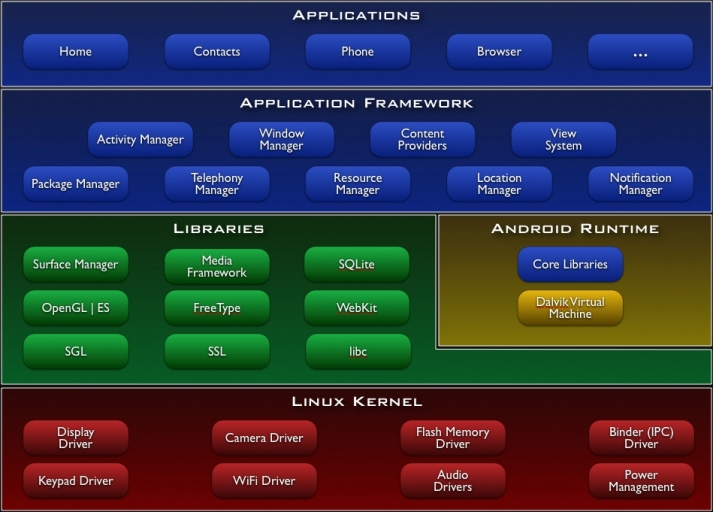
\includegraphics[width=0.9\textwidth]{android_system_architecture.jpg}
			\caption{Αρχιτεκτονική του λειτουργικού συστήματος Android}
			\label{fig:android_system_architecture}
		\end{figure}
		
		 Ξεκινώντας από το χαμηλότερο επίπεδο έχουμε \cite{collinsAndroid}\cite{annuzziAndroid}\cite{androidArchAnalysis}:
		 \begin{itemize}
		 	\item \textbf{Linux Kernel}: ο οποίος είναι ειδικά σχεδιασμένος για το λειτουργικό σύστημα Android και περιέχει τους οδηγούς για το υλικό (κάμερα, πληκτρολόγιο κτλπ). Επίσης ο πυρήνας είναι υπεύθυνος για τη διαχείριση της μνήμης και των διεργασιών, τις συνδέσεις δικτύου και κατ'επέκταση την διαχείριση των διεπαφών δικτύου που διαθέτει κάθε συσκευή. Επιπρόσθετα χειρίζεται τους πόρους και την ενεργεία κάτι το οποίο είναι πολύ σημαντικό δεδομένου της περιορισμένης παροχής ενέργειας των κινητών συσκευών. 
		 	\item \textbf{Libraries} Στο αμέσως επόμενο επίπεδο έχουμε τις βιβλιοθηκές του συστήματος, οι οποίες πολλές φορές αποκαλούνται και εγγενείς βιβλιοθήκες (Native Libraries). Οι εν λόγω βιβλιοθήκες έχουν αναπτυχθεί με χρήση των γλωσσών προγραμματισμού C και C++. Μερικές από τις πιο σημαντικές βιβλιοθήκες αυτού του επίπεδου είναι:
		 	\begin{itemize}
		 		\item WebKit, για την υποστήριξη των φυλλομετρητών
		 		\item Media Framework, για την αναπαραγωγή αρχείων ήχου και βίντεο
		 		\item Surface Manager, για την δημιουργία παραθύρων και ανανέωση της οθόνης
		 		\item SQLite, για την διαχείριση των βάσεων δεδομένων
		 		\item OpenGL, για την απόδοση γραφικών
		 		\item Text, για τον χειρισμό και εμφάνιση κειμένου
		 	\end{itemize}
		 	Σε αυτό το επίπεδο βρίσκεται επίσης και το κομμάτι της εκτέλεσης του Android (Android Runtime), το οποίο υποστηρίζει τη διαδικασία εγγραφής και εκτέλεσης των εφαρμογών. Αποτελείται από δυο βασικές συνιστώσες:
		 	\begin{itemize}
		 		\item Βασικές βιβλιοθήκες για τη διεπαφή των εφαρμογών Java με το περιβάλλον της συσκευής στην οποία εκτελούνται. Πιο αναλυτικά, οι εν λόγω βιβλιοθήκες είναι δυναμικές οι οποίες εισάγονται στην αρχή κάθε κλάσης.
		 		\item Την εικονική μηχανή Dalvik (Dalvik Virtual Machine) η οποία είναι υπεύθυνη για την δημιουργία των εκτελέσιμων αρχείων των εφαρμογών. Συγκεκριμένα ο πηγαίος κώδικας java μετατρέπεται σε μορφή ενδιάμεσου κώδικα (bytecode) και στην συνέχεια μεταφράζεται σε Dalvik bytecode που αποθηκεύεται σε αρχεία της μορφής .dex. Η διαδικασία της μετατροπής των αρχείων κλάσεων java σε μορφή .dex γίνεται από το εργαλείο dx, ενώ παράλληλα γίνεται και βελτιστοποίηση της πλεονάζουσας πληροφορίας με αποτέλεσμα τα αρχεία .dex να είναι μικρότερα σε μέγεθος από τα αντίστοιχα αρχεία κλάσεων. Τέλος το αρχείο .dex μαζί με τους πόρους της εφαρμογής μετατρέπονται σε αρχείο της μορφή .apk (Android Package). Το .apk αρχείο είναι αυτό που χρησιμοποιείται από τον χρήστη για την εγκατάσταση της εφαρμογής στην συσκευή του. Όταν ο χρήστης εκτελέσει την εφαρμογή, τότε η εφαρμογή αυτή θα εκτελεστεί στην εικονική μηχανή Dalvik αντί της JVM, καθώς το περιβάλλον εκτέλεσης των κινητών συσκευών διαθέτει περιορισμένους πόρους.
		 	\end{itemize}
		 	\item \textbf{Application Framework} Στο τρίτο επίπεδο βρίσκεται το πλαίσιο λογισμικού των εφαρμογών, το οποίο ουσιαστικά είναι ένα σύνολο υπηρεσιών οι οποίες δημιουργούν το περιβάλλον μέσα στο οποίο εκτελούνται οι εφαρμογές Android. Μερικές από τις πιο βασικές υπηρεσίες που περιλαμβάνονται στο επίπεδο του applicaiton framework είναι οι παρακάτω:
		 	\begin{itemize}
		 		\item Package Manager: Ο διαχειριστής πακέτων είναι το σύστημα μέσω του οποίου οι εφαρμογές μπορούν να βρουν πληροφορίες για τις υπόλοιπες εφαρμογές που είναι εγκατεστημένες στη συσκευή. Αποτελεί ουσιαστικά μια βάση δεδομένων όλων των εφαρμογών που είναι εγκατεστημένες στην συσκευή και επιτρέπει σε μια μια εφαρμογή να χρησιμοποιήσει μια άλλη και να μοιραστεί δεδομένα με αυτήν.
		 		\item Activity Manager: Ο διαχειριστής δραστηριοτήτων, διαχειρίζεται τον κύκλο ζωής των εφαρμογών και τη στοίβα δραστηριοτήτων (activity stack).
		 		\item Content Providers: Οι πάροχοι περιεχομένου επιτρέπουν στις εφαρμογές να δημοσιεύουν και να μοιράζονται δεδομένα με άλλες εφαρμογές. Αποτελούν ουσιαστικά βάσεις δεδομένων οι οποίες δίνουν την δυνατότητα στις εφαρμογές να αποθηκεύσουν και να μοιραστούν δομημένες πληροφορίες. Παράδειγμα τέτοιων πληροφοριών αποτελούν οι επαφές της συσκευής.
		 		\item View System: Περιλαμβάνει γραφικά στοιχεία τα οποία χρησιμοποιούνται για την δημιουργία της διεπαφής χρήστη. Παράδειγμα γραφικών στοιχείων που περιλαμβάνει είναι κουμπιά, κουτιά κειμένων, πλαίσια κτλπ.
		 		\item Resource Manager: Ο διαχειριστής πόρων είναι υπεύθυνος για την διαχείριση των πόρων που δεν αποτελούν κώδικα και κατ'επέκταση δεν μπορούν να μεταγλωττιστούν. Παράδειγμα τέτοιων στοιχείων αποτελούν τα γραφικά στοιχεία και οι συμβολοσειρές.
		 		\item Notification Manager: Ο διαχειριστής ειδοποιήσεων επιτρέπει στις εφαρμογές να εμφανίζουν ειδοποιήσεις προς το χρήστη. Οι ειδοποιήσεις αυτές εμφανίζονται στην μπάρα κατάστασης της συσκευής η οποία βρίσκεται στο πάνω μέρος της οθόνης και είναι σχεδόν πάντα ορατή στον χρήστη.
		 		\item Telephony Manager: Ο διαχειριστής τηλεφωνίας παρέχει πληροφορίες στην εφαρμογή σχετικά με τις υπηρεσίες τηλεφώνου που είναι διαθέσιμες στην συσκευή.
		 		\item Location Manager: Ο διαχειριστής τοποθεσίας παρέχει στις εφαρμογές πρόσβαση σε πληροφορίες σχετικά με την τοποθεσία και την κίνηση της συσκευής.
		 	\end{itemize}
		 	\item \textbf{Applications} Στο τέταρτο και τελευταίο επίπεδο της αρχιτεκτονικής του λειτουργικού συστήματος Android βρίσκονται οι εφαρμογές. Σε αυτό το επίπεδο περιλαμβάνονται τόσο οι προεγκατεστημένες εφαρμογές όσο και οι εφαρμογές τρίτων.
		 \end{itemize}
		 
		\subsubsection{Δομικά στοιχεία του Android}
		Υπάρχουν τέσσερα βασικά δομικά στοιχεία στο λειτουργικό σύστημα Android (βλ. σχήμα \ref{fig:android_fundamental_components}). Κάθε δομικό στοιχείο επιτελεί ένα ξεχωριστό σκοπό και έχει ανεξάρτητο κύκλο ζωής. Κάθε δομικό στοιχείο αποτελεί ουσιαστικά ένα διαφορετικό σημείο μέσω του οποίου το λειτουργικό σύστημα μπορεί να αποκτήσει πρόσβαση στην εφαρμογή. Στην συνέχεια θα κάνουμε μια συνοπτική παρουσίαση των βασικών αυτών δομικών στοιχειών, θεμελιώνοντας έτσι το θεωρητικό πλαίσιο για ανάπτυξη εφαρμογών Android \cite{androidComponentsKnoxville}\cite{androidFundamentalsOfficial}.
		
		\begin{figure}[h]
			\centering
			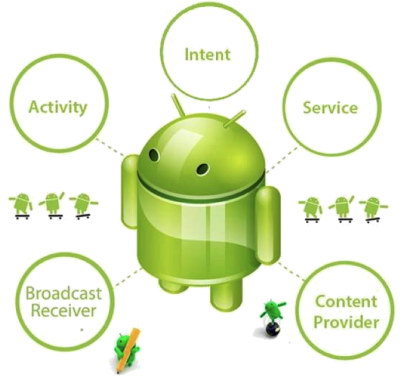
\includegraphics[width=0.6\textwidth]{android_fundamental_components.jpg}
			\caption{Δομικά στοιχεία του Android}
			\label{fig:android_fundamental_components}
		\end{figure}
		
		\subsubsection{Activities}
		Η κλάση Activity αποτελεί την βασικότερη κλάση μιας εφαρμογής Android. Κάθε κλάση Activity αποτελεί μια ξεχωριστή γραφική διεπιφάνεια (παράθυρο/οθόνη) μέσω της οποίας ο χρήστης αλληλεπιδρά με την εφαρμογή. Συνήθως το παράθυρο αυτό καλύπτει όλη την οθόνη της συσκευής αλλά υπάρχουν και κάποιες εξεζητημένες περιπτώσεις στις οποίες καλύπτει μόνο ένας μέρος της οθόνης.
		
		Κάθε εφαρμογή αποτελείται κατά κανόνα από πολλές Activities (οθόνες) οι οποίες είναι συνδεδεμένες μεταξύ τους, ενώ έχουν και την δυνατότητα ανταλλαγής πληροφοριών. Η οθόνη που παρουσιάζεται πρώτη στον χρήστη με το που πραγματοποιήσει εκκίνηση της εφαρμογής ονομάζεται `κύρια' (main), μέσω της οποίας μπορεί να πλοηγηθεί και στις υπόλοιπες οθόνες. Εν γένει κάθε activity έχει την δυνατότητα να πραγματοποιήσει εκκίνηση μια άλλης activity. Το σύστημα κάθε φορά που γίνεται μετάβαση σε μια νέα activity εισχωρεί (push) την προηγούμενη σε μια στοίβα μορφής LIFO που ονομάζεται back-stack, έτσι ώστε αν ο χρήστης πατήσει το κουμπί επιστροφής (back) να μπορεί με ένα pop στην στοίβα να επαναφέρει την αμέσως προηγούμενη activity. Δηλαδή αν ήμασταν αρχικά στην activity Α μέσω της οποία μεταβήκαμε στην Β, η activity Α βρίσκεται στην κορυφή της στοίβας οπότε με το πλήκτρο back οδηγούμαστε πάλι στην οθόνη που βρισκόμασταν προηγουμένως την Α. Σε αυτό το σημείο θα πρέπει να αναφερθεί ότι αν πατηθεί το κουμπί back όταν ο χρήστης βρίσκεται στην αρχική οθόνη και η στοίβα είναι άδεια, πραγματοποιείται έξοδος από την εφαρμογή.
		
		Για την δημιουργία μιας οθόνης θα πρέπει να κάνουμε extend την βασική κλάση Activity και να υλοποιήσουμε κάποιες απαραίτητες μεθόδους της. Συγκεκριμένα κάθε activity  πρέπει να υλοποιεί την μέθοδο onCreate() η οποία καλείται αυτόματα κατά την πρώτη εκκίνηση της activity όπως υπονοεί και το όνομα της. Θα πρέπει να τονιστεί ότι εκτελείται μόνο κατά την πρώτη δημιουργία του activity και όχι όταν επιστρέφουμε σε αυτό με χρήση του κουμπιού της επιστροφής. Μέσα στην εν λόγω μέθοδο γίνεται αρχικοποίηση τον βασικών συστατικών που αποτελούν την διεπαφή του χρήστη.
		
		Μια επίσης εκ των βασικών μεθόδων που πρέπει να υλοποιήσουμε αποτελεί το onPause(). Όπως υποδηλώνει και το όνομά της καλείται από το σύστημα όταν ο χρήστης πραγματοποιεί έξοδο από το συγκεκριμένο activity χωρίς όμως να το καταστρέφει, για παράδειγμα όταν κάνει μετάβαση σε άλλο activity της ίδιας εφαρμογής.
		
		Για να πραγματοποιήσουμε τον τερματισμό ενός activity αρκεί να εκτελεστεί η εντολή finish(), αν και συνήθως δεν χρειάζεται να τερματίζουμε εμείς τις acitivities αφού είναι κάτι που αποτελεί ουσιαστικά δικαιοδοσία του Dalvik. Για να γίνουν καλύτερα κατανοητά τα παραπάνω στο σχήμα \ref{fig:activity_lifecycle} βλέπουμε τον κύκλο ζωής των activities και τις αντίστοιχες μεθόδους.
		
		\begin{figure}[h]
			\centering
			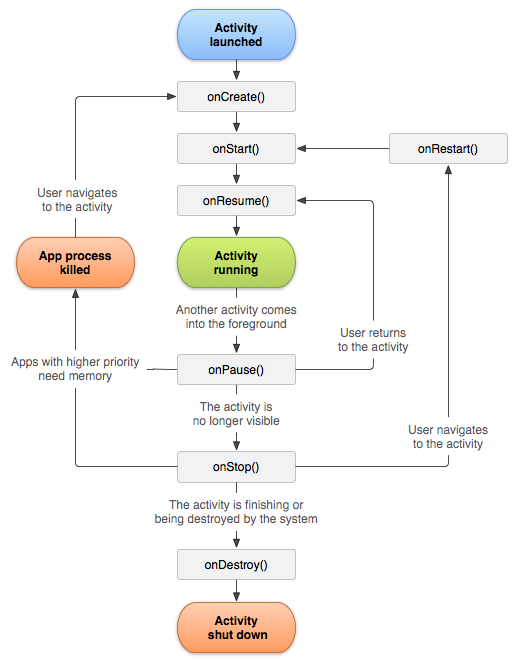
\includegraphics[width=0.5\textwidth]{activity_lifecycle.png}
			\caption{Ο κύκλος ζωής των activities}
			\label{fig:activity_lifecycle}
		\end{figure}
		
		\subsubsection{Services}
		Οι υπηρεσίες αποτελούν τα στοιχεία μιας εφαρμογής οι οποίες εκτελούν χρονοβόρες λειτουργίες στο παρασκήνιο (background) της εφαρμογής. Θεμελιώδη διαφορά μεταξύ μιας υπηρεσίας και ενός activity αποτελεί ότι η υπηρεσία δεν παρέχει κάποια διεπαφή προς τον χρήστη της εφαρμογής, δεδομένου ότι όπως προαναφέρθηκε δρουν παρασκηνιακά. Μια υπηρεσία έχει την δυνατότητα να συνεχίζει την εκτέλεση της στο παρασκήνιο ακόμα και στην περίπτωση όπου ο χρήστης έχει πραγματοποιήσει μετάβαση σε κάποια τελείως διαφορετική εφαρμογή. Ένα κλασσικό παράδειγμα υπηρεσίας αποτελεί η αναπαραγωγή μουσικής, η οποία συνεχίζει να εκτελείται στο παρασκήνιο ακόμα και όταν έχουμε κλείσει την εφαρμογή αναπαραγωγής μουσικής και εκτελούμε τελείως διαφορετικές εφαρμογές. Υπάρχουν κάποιες έτοιμες υπηρεσίες που μας παρέχει το λειτουργικό σύστημα όπως είναι ο Location Manager, αλλά μπορούμε να ορίσουμε και τις δικές μας υπηρεσίες. Μια υπηρεσία μπορεί ουσιαστικά να πάρει δυο διαφορετικές μορφές\cite{servicesAndroid}:
		\begin{itemize}
			\item Started: Μια υπηρεσία έχει εκκινηθεί όταν κάποιο συστατικό της εφαρμογής (π.χ ένα activity) έχει καλέσει την μέθοδο startService(). Μόλις η υπηρεσία εκκινηθεί συνεχίζει να εκτελείται επ' αόριστον στο παρασκήνιο ακόμα και αν το activity που την κάλεσε έχει τερματιστεί. Συνήθως επιτελεί μία και μόνο εργασία χωρίς να επιστρέφει κάποιο αποτέλεσμα στο activity που την κάλεσε. Για παράδειγμα μπορεί να κατεβάζει κάποιο αρχείο και όταν ολοκληρωθεί η μεταφόρτωση του θα τερματίσει η ίδια τον εαυτό της.
			\item Bound: Λέμε ότι μια υπηρεσία είναι `δεμένη' όταν κάποιο συστατικό της εφαρμογής (π.χ ένα activity) έχει καλέσει την μέθοδο bindService(). Μια `δεμένη' υπηρεσία παρέχει διεπαφή πελάτη - εξυπηρετητή (client - server) και επιτρέπει στα συστατικά της εφαρμογής που είναι συνδεδεμένα μαζί της να αλληλεπιδρούν με αυτήν, στέλνοντας αιτήματα και λαμβάνοντας τα αποτελέσματα ακόμα και αν βρίσκονται σε διαφορετικές διεργασίες χρησιμοποιώντας IPC (interprocess communication). Υπηρεσίες τέτοιου τύπου συνεχίζουν την λειτουργία τους όσο τα συστατικά με τα οποία είναι συνδεδεμένα εξακολουθούν να τρέχουν. Η υπηρεσία τερματίζεται μόνο όταν τερματιστεί (ή αποσυνδεθεί) και το τελευταίο συστατικό που είναι συνδεδεμένο με αυτήν.
		\end{itemize}
		Όπως αναφέρθηκε προηγουμένως οι υπηρεσίες δεν παρέχουν κάποια διεπαφή προς τον χρήστη, οπότε δημιουργείται και το εύλογο ερώτημα για το πως θα ενημερώνεται ο χρήστης. Οι υπηρεσίες ειδοποιούν τους χρήστες για τα αποτελέσματα τους είτε με χρήση ειδοποίησης μορφής Toast είτε μέσω ειδοποίησης στο status bar.  Για να γίνουν καλύτερα κατανοητά οι έννοιες που αναλύθηκαν παραπάνω στο σχήμα \ref{fig:service_lifecycle} βλέπουμε τον κύκλο ζωής των υπηρεσιών.
		
		\begin{figure}[h]
			\centering
			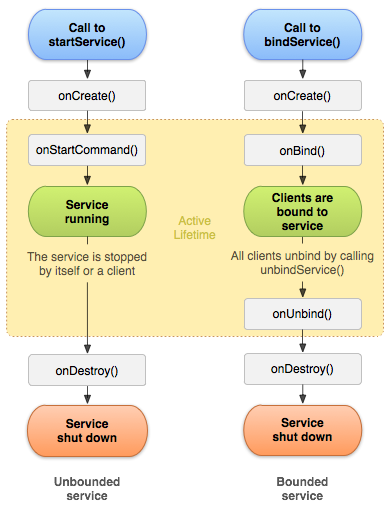
\includegraphics[width=0.5\textwidth]{service_lifecycle.png}
			\caption{Ο κύκλος ζωής των services}
			\label{fig:service_lifecycle}
		\end{figure}
		
		\subsubsection{Content Providers}
		Οι πάροχοι περιεχομένου διαχειρίζονται την πρόσβαση στους αποθηκευτικούς χώρους των δεδομένων. Ουσιαστικά δίνει την δυνατότητα αποθήκευσης και διαμοιρασμού δεδομένων στις εφαρμογές. Ένας πάροχος δεδομένων παρουσιάζει τα δεδομένα στις εφαρμογές σε μορφή πινάκων σαν τους πίνακες σε μια σχεσιακή βάση δεδομένων. Παράδειγμα ενός ενσωματωμένου παροχέα δεδομένων είναι το λεξικό χρήστη στο οποίο αποθηκεύονται οι λέξεις του χρήστη. Για αυτή τη χρήση υπάρχει και η ενσωματωμένη βάση δεδομένων SQLite, η οποία δίνει την δυνατότητα αποθηκεύσης και ανάγνωσης δεδομένων στους παρόχους περιεχομένου.\cite{androidContentProviders}
		\subsubsection{Broadcast Receivers}
		Οι δέκτες εκπεμπόμενων προθέσεων είναι υπεύθυνοι για την λήψη και διαχείριση γεγονότων πραγματοποιούνται στην συσκευή. Συγκεκριμένα ενημερώνονται από το λειτουργικό σύστημα όταν πραγματοποιείται κάποιο γεγονός και τότε ενεργοποιούνται. Χαρακτηριστικά παραδείγματα τέτοιων γεγονότων είναι ότι το κινητό μπήκε σε κατάσταση αναμονής, ότι η στάθμη της μπαταρίας είναι χαμηλή κτλπ. Οι δέκτες εκπεμπόμενων προθέσεων δεν παρέχουν κάποια διεπαφή προς τον χρήστη όπως και οι υπηρεσίες και μπορούν να επικοινωνήσουν με τον χρήστη μέσω ειδοποιήσεων στο status bar.\cite{broadcastReceiver}

		\textbf{Material design ? Αν δεν είναι API Level 21?}
	\subsection{Mockups}
	\subsection{Διασύνδεση με Social Networks}
